% Options for packages loaded elsewhere
\PassOptionsToPackage{unicode}{hyperref}
\PassOptionsToPackage{hyphens}{url}
%
\documentclass[
]{article}
\usepackage{amsmath,amssymb}
\usepackage{iftex}
\ifPDFTeX
  \usepackage[T1]{fontenc}
  \usepackage[utf8]{inputenc}
  \usepackage{textcomp} % provide euro and other symbols
\else % if luatex or xetex
  \usepackage{unicode-math} % this also loads fontspec
  \defaultfontfeatures{Scale=MatchLowercase}
  \defaultfontfeatures[\rmfamily]{Ligatures=TeX,Scale=1}
\fi
\usepackage{lmodern}
\ifPDFTeX\else
  % xetex/luatex font selection
\fi
% Use upquote if available, for straight quotes in verbatim environments
\IfFileExists{upquote.sty}{\usepackage{upquote}}{}
\IfFileExists{microtype.sty}{% use microtype if available
  \usepackage[]{microtype}
  \UseMicrotypeSet[protrusion]{basicmath} % disable protrusion for tt fonts
}{}
\makeatletter
\@ifundefined{KOMAClassName}{% if non-KOMA class
  \IfFileExists{parskip.sty}{%
    \usepackage{parskip}
  }{% else
    \setlength{\parindent}{0pt}
    \setlength{\parskip}{6pt plus 2pt minus 1pt}}
}{% if KOMA class
  \KOMAoptions{parskip=half}}
\makeatother
\usepackage{xcolor}
\usepackage[margin=1in]{geometry}
\usepackage{color}
\usepackage{fancyvrb}
\newcommand{\VerbBar}{|}
\newcommand{\VERB}{\Verb[commandchars=\\\{\}]}
\DefineVerbatimEnvironment{Highlighting}{Verbatim}{commandchars=\\\{\}}
% Add ',fontsize=\small' for more characters per line
\newenvironment{Shaded}{}{}
\newcommand{\AlertTok}[1]{\textcolor[rgb]{1.00,0.00,0.00}{\textbf{#1}}}
\newcommand{\AnnotationTok}[1]{\textcolor[rgb]{0.38,0.63,0.69}{\textbf{\textit{#1}}}}
\newcommand{\AttributeTok}[1]{\textcolor[rgb]{0.49,0.56,0.16}{#1}}
\newcommand{\BaseNTok}[1]{\textcolor[rgb]{0.25,0.63,0.44}{#1}}
\newcommand{\BuiltInTok}[1]{\textcolor[rgb]{0.00,0.50,0.00}{#1}}
\newcommand{\CharTok}[1]{\textcolor[rgb]{0.25,0.44,0.63}{#1}}
\newcommand{\CommentTok}[1]{\textcolor[rgb]{0.38,0.63,0.69}{\textit{#1}}}
\newcommand{\CommentVarTok}[1]{\textcolor[rgb]{0.38,0.63,0.69}{\textbf{\textit{#1}}}}
\newcommand{\ConstantTok}[1]{\textcolor[rgb]{0.53,0.00,0.00}{#1}}
\newcommand{\ControlFlowTok}[1]{\textcolor[rgb]{0.00,0.44,0.13}{\textbf{#1}}}
\newcommand{\DataTypeTok}[1]{\textcolor[rgb]{0.56,0.13,0.00}{#1}}
\newcommand{\DecValTok}[1]{\textcolor[rgb]{0.25,0.63,0.44}{#1}}
\newcommand{\DocumentationTok}[1]{\textcolor[rgb]{0.73,0.13,0.13}{\textit{#1}}}
\newcommand{\ErrorTok}[1]{\textcolor[rgb]{1.00,0.00,0.00}{\textbf{#1}}}
\newcommand{\ExtensionTok}[1]{#1}
\newcommand{\FloatTok}[1]{\textcolor[rgb]{0.25,0.63,0.44}{#1}}
\newcommand{\FunctionTok}[1]{\textcolor[rgb]{0.02,0.16,0.49}{#1}}
\newcommand{\ImportTok}[1]{\textcolor[rgb]{0.00,0.50,0.00}{\textbf{#1}}}
\newcommand{\InformationTok}[1]{\textcolor[rgb]{0.38,0.63,0.69}{\textbf{\textit{#1}}}}
\newcommand{\KeywordTok}[1]{\textcolor[rgb]{0.00,0.44,0.13}{\textbf{#1}}}
\newcommand{\NormalTok}[1]{#1}
\newcommand{\OperatorTok}[1]{\textcolor[rgb]{0.40,0.40,0.40}{#1}}
\newcommand{\OtherTok}[1]{\textcolor[rgb]{0.00,0.44,0.13}{#1}}
\newcommand{\PreprocessorTok}[1]{\textcolor[rgb]{0.74,0.48,0.00}{#1}}
\newcommand{\RegionMarkerTok}[1]{#1}
\newcommand{\SpecialCharTok}[1]{\textcolor[rgb]{0.25,0.44,0.63}{#1}}
\newcommand{\SpecialStringTok}[1]{\textcolor[rgb]{0.73,0.40,0.53}{#1}}
\newcommand{\StringTok}[1]{\textcolor[rgb]{0.25,0.44,0.63}{#1}}
\newcommand{\VariableTok}[1]{\textcolor[rgb]{0.10,0.09,0.49}{#1}}
\newcommand{\VerbatimStringTok}[1]{\textcolor[rgb]{0.25,0.44,0.63}{#1}}
\newcommand{\WarningTok}[1]{\textcolor[rgb]{0.38,0.63,0.69}{\textbf{\textit{#1}}}}
\usepackage{graphicx}
\makeatletter
\def\maxwidth{\ifdim\Gin@nat@width>\linewidth\linewidth\else\Gin@nat@width\fi}
\def\maxheight{\ifdim\Gin@nat@height>\textheight\textheight\else\Gin@nat@height\fi}
\makeatother
% Scale images if necessary, so that they will not overflow the page
% margins by default, and it is still possible to overwrite the defaults
% using explicit options in \includegraphics[width, height, ...]{}
\setkeys{Gin}{width=\maxwidth,height=\maxheight,keepaspectratio}
% Set default figure placement to htbp
\makeatletter
\def\fps@figure{htbp}
\makeatother
\setlength{\emergencystretch}{3em} % prevent overfull lines
\providecommand{\tightlist}{%
  \setlength{\itemsep}{0pt}\setlength{\parskip}{0pt}}
\setcounter{secnumdepth}{-\maxdimen} % remove section numbering
\ifLuaTeX
  \usepackage{selnolig}  % disable illegal ligatures
\fi
\IfFileExists{bookmark.sty}{\usepackage{bookmark}}{\usepackage{hyperref}}
\IfFileExists{xurl.sty}{\usepackage{xurl}}{} % add URL line breaks if available
\urlstyle{same}
\hypersetup{
  hidelinks,
  pdfcreator={LaTeX via pandoc}}

\author{}
\date{}

\begin{document}

\hypertarget{epidemic-data-analysis}{%
\section{epidemic-data-analysis}\label{epidemic-data-analysis}}

Big Data and Data Integration project - S9 GENIOMHE

\textbf{Report on}:
\href{https://raysas.github.io/epidemic-data-analysis/}{\texttt{https://raysas.github.io/epidemic-data-analysis/}}
pages from github:
\href{https://github.com/raysas/epidemic-data-analysis}{\texttt{https://github.com/raysas/epidemic-data-analysis}}.
Provided a web dashboard to visualize the results of the analysis (could
be found on the github link)

\textbf{Tools used}:

\href{https://www.mongodb.com/}{\includegraphics{https://img.shields.io/badge/MongoDB-\%2334A853?logo=mongodb\&logoColor=white}}
\href{https://hadoop.apache.org/}{\includegraphics{https://img.shields.io/badge/Hadoop-\%23EA4335?logo=apachehadoop\&logoColor=white}}
\href{https://plotly.com/dash/}{\includegraphics{https://img.shields.io/badge/Dash-\%23086FA6?logo=plotly\&logoColor=white}}
\href{https://www.python.org/}{\includegraphics{https://img.shields.io/badge/Python-\%233776AB?logo=python\&logoColor=white}}
\href{https://developer.mozilla.org/en-US/docs/Web/JavaScript}{\includegraphics{https://img.shields.io/badge/JavaScript-\%23F7DF1E?logo=javascript\&logoColor=black}}
\href{https://www.docker.com/}{\includegraphics{https://img.shields.io/badge/Docker-\%23007ACC?logo=docker\&logoColor=white}}
\href{https://git-scm.com/}{\includegraphics{https://img.shields.io/badge/Git-\%23F05032?logo=git\&logoColor=white}}

\hypertarget{table-of-contents}{%
\subsection{Table of Contents}\label{table-of-contents}}

\begin{itemize}
\tightlist
\item
  \protect\hyperlink{epidemic-data-analysis}{epidemic-data-analysis}

  \begin{itemize}
  \tightlist
  \item
    \protect\hyperlink{table-of-contents}{Table of Contents}
  \item
    \protect\hyperlink{project-overview}{Project Overview}
  \item
    \protect\hyperlink{environment-setup}{Environment Setup}
  \item
    \protect\hyperlink{mongodb}{MongoDB}

    \begin{itemize}
    \tightlist
    \item
      \protect\hyperlink{1-setup}{1. setup}
    \item
      \protect\hyperlink{2-data-preperation}{2. data preperation}
    \item
      \protect\hyperlink{3-querying}{3. Querying!}

      \begin{itemize}
      \tightlist
      \item
        \protect\hyperlink{31-query-1-continent-stats}{3.1 Query 1:
        Continent stats}
      \item
        \protect\hyperlink{32-query-2-countries-stats}{3.2 Query 2:
        Countries stats}
      \item
        \protect\hyperlink{33-query-3-usa-daily-stats}{3.3 Query 3: USA
        daily stats}
      \item
        \protect\hyperlink{34-query-4-worldwide-daily-stats}{3.4 Query
        4: worldwide daily stats}
      \item
        \protect\hyperlink{35-query-5-casesdeath-weekly-analysis}{3.5
        Query 5: cases/death weekly analysis}
      \item
        \protect\hyperlink{36-query-6-collect-the-14-day-incidence-rate-worldwide-per-day-for-these-2-dates-group-by-country}{3.6
        Query 6: collect the 14-day incidence rate worldwide per day for
        these 2 dates, group by country}
      \end{itemize}
    \end{itemize}
  \item
    \protect\hyperlink{hadoop}{Hadoop}

    \begin{itemize}
    \tightlist
    \item
      \protect\hyperlink{1-setup-1}{1. setup}
    \item
      \protect\hyperlink{2-data-preperation-1}{2. data preperation}
    \item
      \protect\hyperlink{3-queries}{3. Queries}

      \begin{itemize}
      \tightlist
      \item
        \protect\hyperlink{31-query-1-continent-stat}{3.1 Query 1:
        continent stat}
      \item
        \protect\hyperlink{32-query-2-country-stats}{3.2 Query 2:
        country stats}
      \item
        \protect\hyperlink{33-query-3-usa-daily-stats-1}{3.3 Query 3:
        USA daily stats}
      \item
        \protect\hyperlink{34-query-4-worldwide-daily-stats-1}{3.4 Query
        4: worldwide daily stats}
      \item
        \protect\hyperlink{35-query-5}{3.5 Query 5:}
      \item
        \protect\hyperlink{36-query-6}{3.6 Query 6:}
      \end{itemize}
    \end{itemize}
  \item
    \protect\hyperlink{performance-analysis}{Performance Analysis}
  \end{itemize}
\end{itemize}

\hypertarget{project-overview}{%
\subsection{Project Overview}\label{project-overview}}

The project aims to use big data tools to retrieve relevant information
and perform analysis on a large dataset, the data in question is coming
from the
\href{https://www.ecdc.europa.eu/en/publications-data/download-todays-data-geographic-distribution-covid-19-cases-worldwide}{European
Centre for Disease Prevention and Control} and contains daily records of
covid-19 cases and deaths worldwide.

The main steps of the project are:

\begin{itemize}
\tightlist
\item
  Query and processing the data using \textbf{MongoDB} and
  \textbf{Hadoop MapReduce} to retrieve relevant statistics
\item
  Analyze results and visualize them using python
\item
  Compare performance of the two tools
\end{itemize}

\emph{Choice of queries}: my aim here was to retrieve the most diverse
set of statistics possible from the, in a qay that no 2 documents can be
extracted in the same manner, covering as many aggregations as possible.
Secondly, focused on getting a useful type of information that is
relevant to pandamic analysis, such as total cases/deaths per country,
daily cases worldwide, incidence rates, etc. And finally, tried to
diversify the set of visualization used to represent the data, to
highlight the possibilities of dealing with big data, even if the
dataset is not that large (in terms of features`)

This project structure was designed to make it fully accessible and
reprodicible, for that providing a webdashboard, the github repository
and the container used here pushed to docker hub.

\textbf{Directory Structure:}

\begin{Shaded}
\begin{Highlighting}[]
\NormalTok{https://github.com/raysas/epidemic{-}data{-}analysis/}
\NormalTok{├── README.md           \# {-}{-} report file}
\NormalTok{├── TODO.md             \# {-}{-} todo list}
\NormalTok{├── app                 \# {-}{-} dash web dashboard code}
\NormalTok{├── assets              \# {-}{-} images and screenshots}
\NormalTok{├── code                \# {-}{-} data processing and viz code}
\NormalTok{├── data                \# {-}{-} input data files}
\NormalTok{├── figures             \# {-}{-} generated figures and plots}
\NormalTok{├── output              \# {-}{-} output files and documents}
\NormalTok{├── requirements.txt    \# {-}{-} python dependencies for viz and dashboard}
\NormalTok{└── run.py              \# {-}{-} script to run the web dashboard}
\end{Highlighting}
\end{Shaded}

\textbf{For the code:}

Kindly find attached the following directories and subdirectories:

\begin{verbatim}
code/
code/
├── notebooks                 # -- jupyter notebooks for data viz and performance analysis
│   ├── continent_stats.ipynb
│   ├── countries_stats.ipynb
│   ├── daily_stats.ipynb
│   ├── performance_analysis.ipynb
│   ├── start_end_date_incidence_stats.ipynb
│   ├── total_per_country.ipynb
│   └── weekly_stats.ipynb
└── scripts                   # -- scripts for mongodb and hadoop 
    ├── extract_data.sh       # -- commands used to retrieve online data
    ├── mongodb.js            # -- mongodb queries script
    ├── mappers               # -- hadoop mappers
    │   ├── USA_daily_stats_mapper.py
    │   ├── continent_stats_mapper.py
    │   ├── country_stats_mapper.py
    │   ├── start_end_date_incidence_stats_mapper.py
    │   ├── weekly_stats_mapper.py
    │   └── worldwide_daily_stats_mapper.py
    ├── reducers              # -- hadoop reducers 
    │   ├── USA_daily_stats_reducer.py
    │   ├── continent_stats_reducer.py
    │   ├── country_stats_reducer.py
    │   ├── start_end_date_incidence_stats_reducer.py
    │   ├── weekly_stats_reducer.py
    │   └── worldwide_daily_stats_reducer.py
    ├── process_log.py    # -- helper script to process hadoop job logs into metrics
    ├── move_files.sh     # -- helper script to move files into docker containers
    └── split_json.sh     # -- helper script to split large json files
\end{verbatim}

Also attached is the output directory containing main documents:

\begin{verbatim}
output/
utput/
├── hadoop                        // -- csv for each query
│   ├── MR_performance_stats.csv
│   ├── continent_stats.csv
│   ├── country_stats.csv
│   ├── logs                      // -- hadoop job logs for each query
│   │   ├── continent_stats.log
│   │   ├── country_stats.log
│   │   ├── start_end_date_incidence_stats.log
│   │   ├── weekly_stats.log
│   │   └── worldwide_daily_stats.log
│   ├── start_end_date_incidence_stats.csv
│   ├── weekly_stats.csv
│   └── worldwide_daily_stats.csv
└── mongodb                      // -- json for each query              
    ├── USA_daily_stats.json
    ├── continent_stats.json
    ├── country_stats.json
    ├── query_performance_stats.json
    ├── start_end_date_incidence_stats.json
    ├── weekly_stats.json
    └── worldwide_daily_stats.json
\end{verbatim}

\hypertarget{environment-setup}{%
\subsection{Environment Setup}\label{environment-setup}}

For mongodb, used the \texttt{mongo:latest} docker image, for hadoop,
used the \texttt{prasanthj/docker-hadoop} docker image, you can pull the
images corresponding to this project's container from my Docker Hub
repository:
\href{https://hub.docker.com/u/raysas}{raysas/bigdata-geniomhe}.

\hypertarget{mongodb}{%
\subsection{MongoDB}\label{mongodb}}

\begin{quote}
{[}!NOTE{]}\\
All mongodb commands here can be found in a javascript script in
code/scripts/mongodb.js
\end{quote}

\hypertarget{setup}{%
\subsubsection{1. setup}\label{setup}}

\textbf{Starting by setting up a mongodb container using the pulled
image and downloading the dataset}

\begin{Shaded}
\begin{Highlighting}[]
\CommentTok{\#docker pull mongo \#{-}{-} pull the image if not there}
\ExtensionTok{docker}\NormalTok{ run }\AttributeTok{{-}d} \AttributeTok{{-}{-}name}\NormalTok{ bigdata\_mongodb }\AttributeTok{{-}p}\NormalTok{ 27017{-}27019:27017{-}27019 mongo:latest}
\end{Highlighting}
\end{Shaded}

\hypertarget{data-preperation}{%
\subsubsection{2. data preperation}\label{data-preperation}}

\textbf{Importing the datasets into the mongodb container, then using
\texttt{mongoimport} command}

On my local machine: 1. will download the publically available covid-19
dataset: ```bash \# -- installing curl if not there apt-get update \&\&
apt-get install -y curl

\begin{verbatim}
# -- downloading the dataset first 
curl https://opendata.ecdc.europa.eu/covid19/casedistribution/json/data.json -o data/covid.json
```
\end{verbatim}

\begin{enumerate}
\def\labelenumi{\arabic{enumi}.}
\setcounter{enumi}{1}
\item
  will split the data into 2 files \emph{p.s. wrote a script to split
  the json into 2 files as the file is 26Mb surpassing the 16Mb limit of
  mongodb import (you can find it in
  \texttt{code/scripts/split\_json.sh})}

\begin{Shaded}
\begin{Highlighting}[]
\ExtensionTok{./code/scripts/split\_json.sh}\NormalTok{ data/covid.json 2 }
\FunctionTok{ls}\NormalTok{ data/}
\end{Highlighting}
\end{Shaded}

  Now will have \texttt{data/covid\_part\_1.json} and
  \texttt{data/covid\_part\_2.json} files each less than 16Mb
\item
  copy the files to docker container
  \texttt{bash\ \ \ \ \ docker\ cp\ data/covid\_part\_1.json\ bigdata\_mongodb:/data/covid\_part\_1.json\ \ \ \ \ docker\ cp\ data/covid\_part\_2.json\ bigdata\_mongodb:/data/covid\_part\_2.json}
\end{enumerate}

\emph{entering the container now}

\begin{Shaded}
\begin{Highlighting}[]
\ExtensionTok{docker}\NormalTok{ exec }\AttributeTok{{-}it}\NormalTok{ bigdata\_mongodb bash}

\CommentTok{\# {-}{-} importing the data into mongodb}
\ExtensionTok{mongoimport} \AttributeTok{{-}{-}db}\NormalTok{ covid\_db }\AttributeTok{{-}{-}collection}\NormalTok{ worldwide\_cases }\AttributeTok{{-}{-}file}\NormalTok{ data/covid\_part\_1.json }\AttributeTok{{-}{-}jsonArray}
\ExtensionTok{mongoimport} \AttributeTok{{-}{-}db}\NormalTok{ covid\_db }\AttributeTok{{-}{-}collection}\NormalTok{ worldwide\_cases }\AttributeTok{{-}{-}file}\NormalTok{ data/covid\_part\_2.json }\AttributeTok{{-}{-}jsonArray}
\end{Highlighting}
\end{Shaded}

\hypertarget{querying}{%
\subsubsection{3. Querying!}\label{querying}}

\emph{entering mongo shell now}

\begin{Shaded}
\begin{Highlighting}[]
\ExtensionTok{mongosh}
\ExtensionTok{use}\NormalTok{ covid\_db}
\ExtensionTok{show}\NormalTok{ collections}
\end{Highlighting}
\end{Shaded}

\textbf{General Data Queries}

\begin{Shaded}
\begin{Highlighting}[]
\CommentTok{// {-}{-} count the number of documents in the collection}
\NormalTok{db}\OperatorTok{.}\AttributeTok{worldwide\_cases}\OperatorTok{.}\FunctionTok{countDocuments}\NormalTok{()}
\CommentTok{// 61900}

\CommentTok{// {-}{-} find one document to see the structure}
\NormalTok{db}\OperatorTok{.}\AttributeTok{worldwide\_cases}\OperatorTok{.}\FunctionTok{findOne}\NormalTok{(\{\})}
\end{Highlighting}
\end{Shaded}

\begin{Shaded}
\begin{Highlighting}[]
\FunctionTok{\{}
  \ErrorTok{\_id}\FunctionTok{:} \ErrorTok{ObjectId(\textquotesingle{}}\DecValTok{690}\ErrorTok{f33b777a56eeaf189a2dd\textquotesingle{})}\FunctionTok{,}
  \ErrorTok{dateRep}\FunctionTok{:} \ErrorTok{\textquotesingle{}}\DecValTok{03}\ErrorTok{/}\DecValTok{12}\ErrorTok{/}\DecValTok{2020}\ErrorTok{\textquotesingle{}}\FunctionTok{,}
  \ErrorTok{day}\FunctionTok{:} \ErrorTok{\textquotesingle{}}\DecValTok{03}\ErrorTok{\textquotesingle{}}\FunctionTok{,}
  \ErrorTok{month}\FunctionTok{:} \ErrorTok{\textquotesingle{}}\DecValTok{12}\ErrorTok{\textquotesingle{}}\FunctionTok{,}
  \ErrorTok{year}\FunctionTok{:} \ErrorTok{\textquotesingle{}}\DecValTok{2020}\ErrorTok{\textquotesingle{}}\FunctionTok{,}
  \ErrorTok{cases}\FunctionTok{:} \DecValTok{202}\FunctionTok{,}
  \ErrorTok{deaths}\FunctionTok{:} \DecValTok{19}\FunctionTok{,}
  \ErrorTok{countriesAndTerritories}\FunctionTok{:} \ErrorTok{\textquotesingle{}Afghanistan\textquotesingle{}}\FunctionTok{,}
  \ErrorTok{geoId}\FunctionTok{:} \ErrorTok{\textquotesingle{}AF\textquotesingle{}}\FunctionTok{,}
  \ErrorTok{countryterritoryCode}\FunctionTok{:} \ErrorTok{\textquotesingle{}AFG\textquotesingle{}}\FunctionTok{,}
  \ErrorTok{popData2019}\FunctionTok{:} \DecValTok{38041757}\FunctionTok{,}
  \ErrorTok{continentExp}\FunctionTok{:} \ErrorTok{\textquotesingle{}Asia\textquotesingle{}}\FunctionTok{,}
  \ErrorTok{\textquotesingle{}Cumulative\_number\_for\_14\_days\_of\_COVID{-}19\_cases\_per\_100000\textquotesingle{}}\FunctionTok{:} \ErrorTok{\textquotesingle{}}\FloatTok{7.53645527}\ErrorTok{\textquotesingle{}}
\FunctionTok{\}}
\end{Highlighting}
\end{Shaded}

\begin{Shaded}
\begin{Highlighting}[]
\CommentTok{// {-}{-} number of countries enlisted}
\NormalTok{db}\OperatorTok{.}\AttributeTok{worldwide\_cases}\OperatorTok{.}\FunctionTok{distinct}\NormalTok{(}\StringTok{"countriesAndTerritories"}\NormalTok{)}\OperatorTok{.}\AttributeTok{length}
\CommentTok{// 214}
\end{Highlighting}
\end{Shaded}

We notice that we can perform soem preprocessing on the data:

\begin{itemize}
\tightlist
\item
  the
  \texttt{Cumulative\_number\_for\_14\_days\_of\_COVID-19\_cases\_per\_100000}
  field is a string, better to convert it into a double
\item
  date is in \texttt{dd/mm/yyyy} format, might be better to convert it
  into a date object for easier querying and processing later on (step2)
\end{itemize}

\begin{Shaded}
\begin{Highlighting}[]
\NormalTok{db}\OperatorTok{.}\AttributeTok{worldwide\_cases}\OperatorTok{.}\FunctionTok{updateMany}\NormalTok{(\{\}}\OperatorTok{,} 
\NormalTok{  [\{ }\DataTypeTok{$set}\OperatorTok{:} 
\NormalTok{    \{ }
      \StringTok{"Cumulative\_number\_for\_14\_days\_of\_COVID{-}19\_cases\_per\_100000"}\OperatorTok{:} 
\NormalTok{          \{ }\DataTypeTok{$convert}\OperatorTok{:}\NormalTok{ \{}
            \DataTypeTok{input}\OperatorTok{:} \StringTok{"$Cumulative\_number\_for\_14\_days\_of\_COVID{-}19\_cases\_per\_100000"}\OperatorTok{,}
            \DataTypeTok{to}\OperatorTok{:} \StringTok{"double"}\OperatorTok{,}
            \DataTypeTok{onError}\OperatorTok{:} \KeywordTok{null}\OperatorTok{,}
            \DataTypeTok{onNull}\OperatorTok{:} \KeywordTok{null}
\NormalTok{          \}}
\NormalTok{    \} }
\NormalTok{\} \} ])}\OperatorTok{;}

\NormalTok{db}\OperatorTok{.}\AttributeTok{worldwide\_cases}\OperatorTok{.}\FunctionTok{updateMany}\NormalTok{(}
\NormalTok{  \{\}}\OperatorTok{,}\NormalTok{[}
\NormalTok{    \{ }
      \DataTypeTok{$set}\OperatorTok{:}\NormalTok{ \{ }
        \DataTypeTok{date}\OperatorTok{:}\NormalTok{ \{}
          \DataTypeTok{$dateFromString}\OperatorTok{:}\NormalTok{ \{ }\DataTypeTok{dateString}\OperatorTok{:} \StringTok{"$dateRep"}\OperatorTok{,} \DataTypeTok{format}\OperatorTok{:} \StringTok{"\%d/\%m/\%Y"}\NormalTok{ \}}
\NormalTok{        \}}
\NormalTok{      \}\}}
\NormalTok{])}\OperatorTok{;}
\end{Highlighting}
\end{Shaded}

This helper function is used at each step to save the results of the
queries into json files:

\begin{Shaded}
\begin{Highlighting}[]
\CommentTok{// {-}{-} helper function to save a json file from a cursor}
\KeywordTok{function} \FunctionTok{save\_json\_file}\NormalTok{(cursor}\OperatorTok{,}\NormalTok{ filename) \{}
    \KeywordTok{var}\NormalTok{ array\_data }\OperatorTok{=}\NormalTok{ []}
    \ControlFlowTok{while}\NormalTok{ (cursor}\OperatorTok{.}\FunctionTok{hasNext}\NormalTok{()) \{}
\NormalTok{        array\_data}\OperatorTok{.}\FunctionTok{push}\NormalTok{(cursor}\OperatorTok{.}\FunctionTok{next}\NormalTok{())}
\NormalTok{    \}}
    \KeywordTok{var}\NormalTok{ file\_data }\OperatorTok{=} \BuiltInTok{JSON}\OperatorTok{.}\FunctionTok{stringify}\NormalTok{(array\_data}\OperatorTok{,} \KeywordTok{null}\OperatorTok{,} \DecValTok{2}\NormalTok{)}
    \KeywordTok{const}\NormalTok{ fs }\OperatorTok{=} \PreprocessorTok{require}\NormalTok{(}\StringTok{\textquotesingle{}fs\textquotesingle{}}\NormalTok{)}\OperatorTok{;}
\NormalTok{    fs}\OperatorTok{.}\FunctionTok{writeFileSync}\NormalTok{(filename}\OperatorTok{,}\NormalTok{ file\_data)}\OperatorTok{;}
    \FunctionTok{print}\NormalTok{(}\VerbatimStringTok{\textasciigrave{}{-}{-} json file saved in: }\SpecialCharTok{$\{}\NormalTok{filename}\SpecialCharTok{\}}\VerbatimStringTok{\textasciigrave{}}\NormalTok{)}
\NormalTok{\}}
\end{Highlighting}
\end{Shaded}

\hypertarget{query-1-continent-stats}{%
\paragraph{3.1 Query 1: Continent stats}\label{query-1-continent-stats}}

\textbf{about}: collecting metrics across continents such as total
cases, total deaths, number of countries and average 14-day incidence
rate\\
\textbf{how?}: using mongodb aggregation framework, will first group by
country to get total cases/deaths and average incidence rate per
country, then group by continent to get the final stats. Aggregation for
cases, deaths and number of countries is done using \texttt{\$sum}
operator, while average incidence rate is done using \texttt{\$avg}
operator\\
\textbf{aim}: get a high level overview of the pandemic situation across
continents, first larger scale look at the data distribution

\begin{quote}
whats new: performing 2 consecutive group stages to get the desired
result
\end{quote}

\begin{Shaded}
\begin{Highlighting}[]
\CommentTok{// 0) data distribution over continents}
\NormalTok{continent\_stats}\OperatorTok{=}\NormalTok{db}\OperatorTok{.}\AttributeTok{worldwide\_cases}\OperatorTok{.}\FunctionTok{aggregate}\NormalTok{([}
\NormalTok{  \{}
    \DataTypeTok{$group}\OperatorTok{:}\NormalTok{ \{}
      \DataTypeTok{\_id}\OperatorTok{:} \StringTok{"$countriesAndTerritories"}\OperatorTok{,}
      \DataTypeTok{continent}\OperatorTok{:}\NormalTok{ \{ }\DataTypeTok{$first}\OperatorTok{:} \StringTok{"$continentExp"}\NormalTok{ \}}\OperatorTok{,}
      \DataTypeTok{avg14DayIncidence}\OperatorTok{:}\NormalTok{ \{ }\DataTypeTok{$avg}\OperatorTok{:} \StringTok{"$Cumulative\_number\_for\_14\_days\_of\_COVID{-}19\_cases\_per\_100000"}\NormalTok{ \}}\OperatorTok{,}
      \DataTypeTok{totalCases}\OperatorTok{:}\NormalTok{ \{ }\DataTypeTok{$sum}\OperatorTok{:} \StringTok{"$cases"}\NormalTok{ \}}\OperatorTok{,}
      \DataTypeTok{totalDeaths}\OperatorTok{:}\NormalTok{ \{ }\DataTypeTok{$sum}\OperatorTok{:} \StringTok{"$deaths"}\NormalTok{ \}}
\NormalTok{    \}}
\NormalTok{  \}}\OperatorTok{,}
\NormalTok{  \{ }\DataTypeTok{$group}\OperatorTok{:}\NormalTok{ \{}
      \DataTypeTok{\_id}\OperatorTok{:} \StringTok{"$continent"}\OperatorTok{,}
      \DataTypeTok{totalCases}\OperatorTok{:}\NormalTok{ \{ }\DataTypeTok{$sum}\OperatorTok{:} \StringTok{"$totalCases"}\NormalTok{ \}}\OperatorTok{,}
      \DataTypeTok{totalDeaths}\OperatorTok{:}\NormalTok{ \{ }\DataTypeTok{$sum}\OperatorTok{:} \StringTok{"$totalDeaths"}\NormalTok{ \}}\OperatorTok{,}
      \DataTypeTok{numberOfCountries}\OperatorTok{:}\NormalTok{ \{ }\DataTypeTok{$sum}\OperatorTok{:} \DecValTok{1}\NormalTok{ \}}\OperatorTok{,}
      \DataTypeTok{avg14DayIncidence}\OperatorTok{:}\NormalTok{ \{ }\DataTypeTok{$avg}\OperatorTok{:} \StringTok{"$avg14DayIncidence"}\NormalTok{ \}}
\NormalTok{    \}}
\NormalTok{  \}}\OperatorTok{,}
\NormalTok{  \{ }\DataTypeTok{$project}\OperatorTok{:}\NormalTok{ \{}
      \DataTypeTok{continent}\OperatorTok{:} \StringTok{"$\_id"}\OperatorTok{,}
      \DataTypeTok{totalCases}\OperatorTok{:} \DecValTok{1}\OperatorTok{,}
      \DataTypeTok{totalDeaths}\OperatorTok{:} \DecValTok{1}\OperatorTok{,}
      \DataTypeTok{numberOfCountries}\OperatorTok{:} \DecValTok{1}\OperatorTok{,}
      \DataTypeTok{avg14DayIncidence}\OperatorTok{:} \DecValTok{1}
\NormalTok{    \}}
\NormalTok{  \}}\OperatorTok{,}
\NormalTok{  \{ }\DataTypeTok{$sort}\OperatorTok{:}\NormalTok{ \{ }\DataTypeTok{totalCases}\OperatorTok{:} \OperatorTok{{-}}\DecValTok{1}\NormalTok{ \} \}}
\NormalTok{])}
\end{Highlighting}
\end{Shaded}

\begin{quote}
{[}!NOTE{]} after each step we run:
\end{quote}

\begin{Shaded}
\begin{Highlighting}[]
\CommentTok{// {-}{-} performance analysis}
\KeywordTok{var}\NormalTok{ continent\_stats\_performance}\OperatorTok{=}\NormalTok{db}\OperatorTok{.}\AttributeTok{worldwide\_cases}\OperatorTok{.}\FunctionTok{aggregate}\NormalTok{([}
\NormalTok{  \{}
    \DataTypeTok{$group}\OperatorTok{:}\NormalTok{ \{}
      \DataTypeTok{\_id}\OperatorTok{:} \StringTok{"$countriesAndTerritories"}\OperatorTok{,}
      \DataTypeTok{continent}\OperatorTok{:}\NormalTok{ \{ }\DataTypeTok{$first}\OperatorTok{:} \StringTok{"$continentExp"}\NormalTok{ \}}\OperatorTok{,}
      \DataTypeTok{avg14DayIncidence}\OperatorTok{:}\NormalTok{ \{ }\DataTypeTok{$avg}\OperatorTok{:} \StringTok{"$Cumulative\_number\_for\_14\_days\_of\_COVID{-}19\_cases\_per\_100000"}\NormalTok{ \}}\OperatorTok{,}
      \DataTypeTok{totalCases}\OperatorTok{:}\NormalTok{ \{ }\DataTypeTok{$sum}\OperatorTok{:} \StringTok{"$cases"}\NormalTok{ \}}\OperatorTok{,}
      \DataTypeTok{totalDeaths}\OperatorTok{:}\NormalTok{ \{ }\DataTypeTok{$sum}\OperatorTok{:} \StringTok{"$deaths"}\NormalTok{ \}}
\NormalTok{    \}}
\NormalTok{  \}}\OperatorTok{,}
\NormalTok{  \{ }\DataTypeTok{$group}\OperatorTok{:}\NormalTok{ \{}
      \DataTypeTok{\_id}\OperatorTok{:} \StringTok{"$continent"}\OperatorTok{,}
      \DataTypeTok{totalCases}\OperatorTok{:}\NormalTok{ \{ }\DataTypeTok{$sum}\OperatorTok{:} \StringTok{"$totalCases"}\NormalTok{ \}}\OperatorTok{,}
      \DataTypeTok{totalDeaths}\OperatorTok{:}\NormalTok{ \{ }\DataTypeTok{$sum}\OperatorTok{:} \StringTok{"$totalDeaths"}\NormalTok{ \}}\OperatorTok{,}
      \DataTypeTok{numberOfCountries}\OperatorTok{:}\NormalTok{ \{ }\DataTypeTok{$sum}\OperatorTok{:} \DecValTok{1}\NormalTok{ \}}\OperatorTok{,}
      \DataTypeTok{avg14DayIncidence}\OperatorTok{:}\NormalTok{ \{ }\DataTypeTok{$avg}\OperatorTok{:} \StringTok{"$avg14DayIncidence"}\NormalTok{ \}}
\NormalTok{    \}}
\NormalTok{  \}}\OperatorTok{,}
\NormalTok{  \{ }\DataTypeTok{$project}\OperatorTok{:}\NormalTok{ \{}
      \DataTypeTok{continent}\OperatorTok{:} \StringTok{"$\_id"}\OperatorTok{,}
      \DataTypeTok{totalCases}\OperatorTok{:} \DecValTok{1}\OperatorTok{,}
      \DataTypeTok{totalDeaths}\OperatorTok{:} \DecValTok{1}\OperatorTok{,}
      \DataTypeTok{numberOfCountries}\OperatorTok{:} \DecValTok{1}\OperatorTok{,}
      \DataTypeTok{avg14DayIncidence}\OperatorTok{:} \DecValTok{1}
\NormalTok{    \}}
\NormalTok{  \}}\OperatorTok{,}

\NormalTok{  \{ }\DataTypeTok{$sort}\OperatorTok{:}\NormalTok{ \{ }\DataTypeTok{totalCases}\OperatorTok{:} \OperatorTok{{-}}\DecValTok{1}\NormalTok{ \} \}}
\NormalTok{])}\OperatorTok{.}\FunctionTok{explain}\NormalTok{(}\StringTok{"executionStats"}\NormalTok{)}
\KeywordTok{var}\NormalTok{ cursorStage }\OperatorTok{=}\NormalTok{ continent\_stats\_performance}\OperatorTok{.}\AttributeTok{stages}\NormalTok{[}\DecValTok{0}\NormalTok{][}\StringTok{\textquotesingle{}$cursor\textquotesingle{}}\NormalTok{]}\OperatorTok{.}\AttributeTok{executionStats}\OperatorTok{;}

\KeywordTok{var}\NormalTok{ queryStatsDoc }\OperatorTok{=}\NormalTok{ \{}
    \DataTypeTok{query\_name}\OperatorTok{:} \StringTok{"continent\_stats"}\OperatorTok{,}  
    \DataTypeTok{executionTimeMillis}\OperatorTok{:}\NormalTok{ cursorStage}\OperatorTok{.}\AttributeTok{executionTimeMillis}\OperatorTok{,}
    \DataTypeTok{totalDocsExamined}\OperatorTok{:}\NormalTok{ cursorStage}\OperatorTok{.}\AttributeTok{totalDocsExamined}\OperatorTok{,}
    \DataTypeTok{nReturned}\OperatorTok{:}\NormalTok{ cursorStage}\OperatorTok{.}\AttributeTok{nReturned}\OperatorTok{,}
    \DataTypeTok{timestamp}\OperatorTok{:} \KeywordTok{new} \BuiltInTok{Date}\NormalTok{() }
\NormalTok{\}}\OperatorTok{;}

\NormalTok{db}\OperatorTok{.}\AttributeTok{query\_performance}\OperatorTok{.}\FunctionTok{insertOne}\NormalTok{(queryStatsDoc)}\OperatorTok{;}
\NormalTok{db}\OperatorTok{.}\AttributeTok{query\_performance}\OperatorTok{.}\FunctionTok{find}\NormalTok{()}\OperatorTok{;}
\end{Highlighting}
\end{Shaded}

This allows us to log the performance of each query into a separate
collection for later analysis and comparison with hadoop. At the end of
all queries, we will have a \texttt{query\_performance\_stats}
collection containing the execution time and number of documents
examined for each query (you can find it in
\texttt{output/mongodb/query\_performance\_stats.json})

The result will be a set of documents having these fields:

\begin{itemize}
\tightlist
\item
  \texttt{\_id}: continent name
\item
  \texttt{totalCases}: total number of cases in the continent
\item
  \texttt{totalDeaths}: total number of deaths in the continent
\item
  \texttt{numberOfCountries}: number of countries in the continent
\item
  \texttt{avg14DayIncidence}: average 14-day incidence rate across
  countries in the continent
\end{itemize}

\begin{figure}
\centering
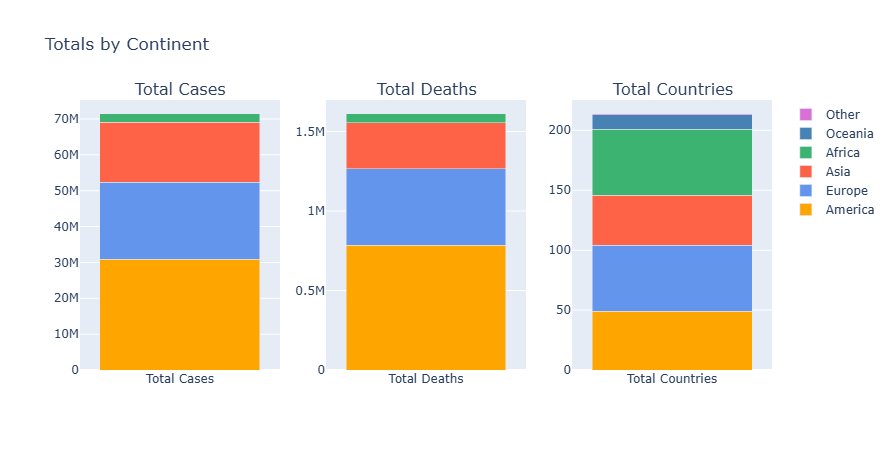
\includegraphics{./figures/mongodb/mongodb_continent_dist.png}
\caption{MongoDB: Stacked bar plot showing distribution accross
continents}
\end{figure}

The \textbf{stacked bar plot} above shows the distribution of total
cases and total deaths accross continents, we can see that Europe and
North America are the most affected continents in terms of total cases
and deaths, followed by Asia and South America. Africa is the least
affected continent, even though it has a large number of countries. This
might be an indicator of underreporting or lack of testing in Africa
compared to other continents, or it could be due to other factors such
as demographics, healthcare infrastructure, or even the fact that the
pandemic reached Africa later than other continents.

\hypertarget{query-2-countries-stats}{%
\paragraph{3.2 Query 2: Countries stats}\label{query-2-countries-stats}}

\textbf{about}: collecting metrics per country such as total cases,
total deaths, population and percentages of cases and deaths relative to
population\\
\textbf{how?}: using mongodb aggregation, will group by country to get
total cases/deaths and population, then calculate percentages using
\texttt{\$addFields} stage\\
\textbf{aim}: get a detailed overview of the pandemic situation per
country

\begin{quote}
whats new: performing normalization of cases and deaths by population
size getting use of 2 fields to create a 3rd one, good to make them
comparable accross countries (especially for heatmap viz)
\end{quote}

\begin{Shaded}
\begin{Highlighting}[]
\CommentTok{// 1) map per country}
\NormalTok{country\_stats }\OperatorTok{=}\NormalTok{ db}\OperatorTok{.}\AttributeTok{worldwide\_cases}\OperatorTok{.}\FunctionTok{aggregate}\NormalTok{([}
\NormalTok{  \{}
    \DataTypeTok{$group}\OperatorTok{:}\NormalTok{ \{}
      \DataTypeTok{\_id}\OperatorTok{:} \StringTok{"$countriesAndTerritories"}\OperatorTok{,}
      \DataTypeTok{geoId}\OperatorTok{:}\NormalTok{ \{ }\DataTypeTok{$first}\OperatorTok{:} \StringTok{"$geoId"}\NormalTok{ \}}\OperatorTok{,}
      \DataTypeTok{totalCases}\OperatorTok{:}\NormalTok{ \{ }\DataTypeTok{$sum}\OperatorTok{:} \StringTok{"$cases"}\NormalTok{ \}}\OperatorTok{,}
      \DataTypeTok{totalDeaths}\OperatorTok{:}\NormalTok{ \{ }\DataTypeTok{$sum}\OperatorTok{:} \StringTok{"$deaths"}\NormalTok{ \}}\OperatorTok{,}
      \DataTypeTok{popData2019}\OperatorTok{:}\NormalTok{ \{ }\DataTypeTok{$first}\OperatorTok{:}\NormalTok{ \{ }\DataTypeTok{$toInt}\OperatorTok{:} \StringTok{"$popData2019"}\NormalTok{ \}\}}\OperatorTok{,}
      \DataTypeTok{avg14DayIncidence}\OperatorTok{:}\NormalTok{ \{ }\DataTypeTok{$avg}\OperatorTok{:} \StringTok{"$Cumulative\_number\_for\_14\_days\_of\_COVID{-}19\_cases\_per\_100000"}
\NormalTok{    \}}
\NormalTok{    \}}
\NormalTok{  \}}\OperatorTok{,}
\NormalTok{  \{}
    \DataTypeTok{$addFields}\OperatorTok{:}\NormalTok{ \{}
      \DataTypeTok{percTotalCases}\OperatorTok{:}\NormalTok{ \{ }\DataTypeTok{$multiply}\OperatorTok{:}\NormalTok{ [ \{ }\DataTypeTok{$divide}\OperatorTok{:}\NormalTok{ [}\StringTok{"$totalCases"}\OperatorTok{,} \StringTok{"$popData2019"}\NormalTok{] \}}\OperatorTok{,} \DecValTok{100}\NormalTok{ ] \}}\OperatorTok{,}
      \DataTypeTok{percTotalDeaths}\OperatorTok{:}\NormalTok{ \{ }\DataTypeTok{$multiply}\OperatorTok{:}\NormalTok{ [ \{ }\DataTypeTok{$divide}\OperatorTok{:}\NormalTok{ [}\StringTok{"$totalDeaths"}\OperatorTok{,} \StringTok{"$popData2019"}\NormalTok{] \}}\OperatorTok{,} \DecValTok{100}\NormalTok{ ] \}}\OperatorTok{,}
\NormalTok{    \}}
\NormalTok{  \}}
\NormalTok{])}
\end{Highlighting}
\end{Shaded}

Result:

\begin{itemize}
\tightlist
\item
  \texttt{\_id}: country name
\item
  \texttt{geoId}: country geo id
\item
  \texttt{totalCases}: total number of cases in the country
\item
  \texttt{totalDeaths}: total number of deaths in the country
\item
  \texttt{popData2019}: country population in 2019
\item
  \texttt{percTotalCases}: percentage of total cases relative to
  population
\item
  \texttt{percTotalDeaths}: percentage of total deaths relative to
  population
\item
  \texttt{avg14DayIncidence}: average 14-day incidence rate in the
  country
\end{itemize}

\begin{figure}
\centering
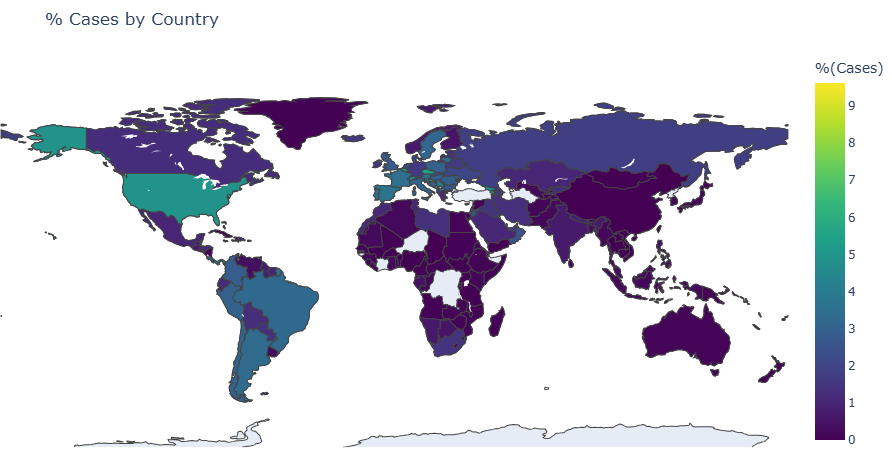
\includegraphics{./figures/mongodb/mongodb_countries_casesc.png}
\caption{MongoDB: map showing percentage of cases relative to population
per country}
\end{figure}

\begin{figure}
\centering
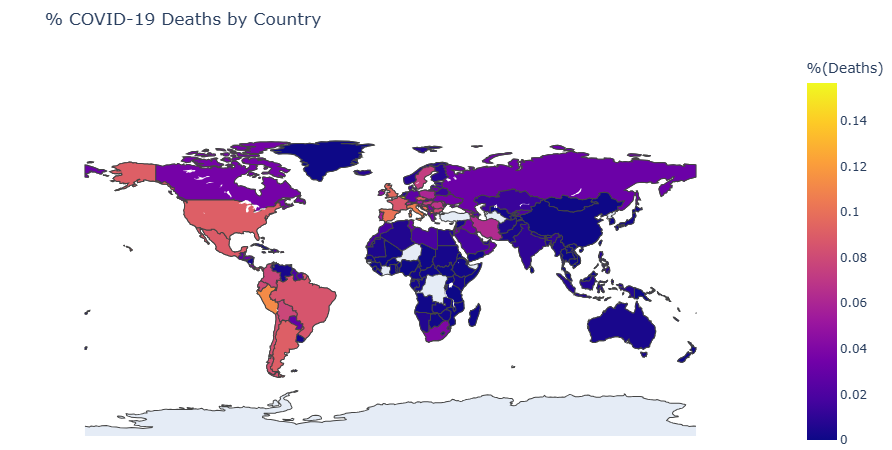
\includegraphics{./figures/mongodb/mongodb_countries_deathc.png}
\caption{MongoDB: map showing percentage of deaths relative to
population per country}
\end{figure}

\begin{figure}
\centering
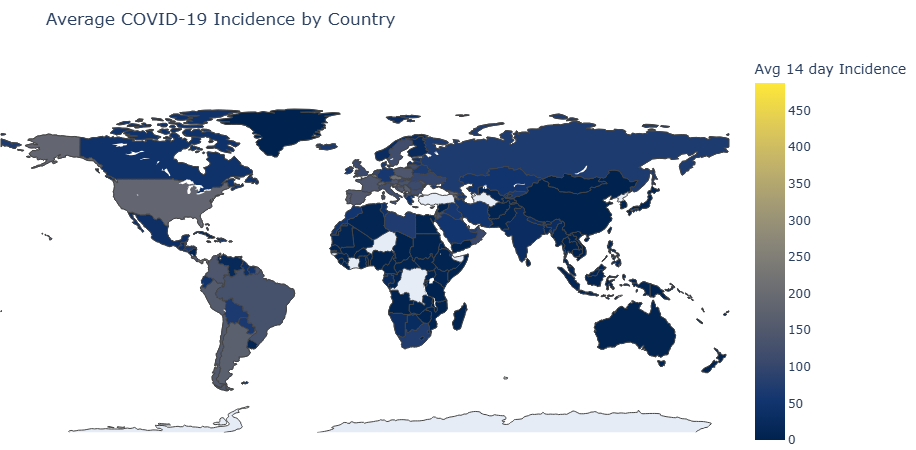
\includegraphics{./figures/mongodb/mongodb_countries_incidence.png}
\caption{MongoDB: map showing average 14-day incidence rate per country}
\end{figure}

\emph{Here used the pycountry library in python to convert country names
to map geoId to their corresponding 3-letter country codes (for plotly
map visualization)}

\hypertarget{query-3-usa-daily-stats}{%
\paragraph{3.3 Query 3: USA daily stats}\label{query-3-usa-daily-stats}}

\textbf{about}: collecting daily total cases and deaths for the USA,
along with cumulative cases and deaths over time \textbf{how?}: using
mongodb aggregation, will first filter for USA records, then group by
date to get total cases/deaths per day, finally use
\texttt{\$setWindowFields} stage to calculate cumulative cases/deaths
over time \textbf{aim}: get a time series of the pandemic situation in
the USA, one of the most affected countries

\begin{quote}
whats new: using \texttt{\$setWindowFields} stage to calculate
cumulative sums over time, useful for time series analysis. Also needing
to match first before grouping (only usa)
\end{quote}

\begin{Shaded}
\begin{Highlighting}[]
\NormalTok{db}\OperatorTok{.}\AttributeTok{worldwide\_cases}\OperatorTok{.}\FunctionTok{find}\NormalTok{(\{ }\DataTypeTok{geoId}\OperatorTok{:} \StringTok{"US"}\NormalTok{ \})}\OperatorTok{.}\FunctionTok{limit}\NormalTok{(}\DecValTok{1}\NormalTok{)}
\NormalTok{country\_daily\_stats}\OperatorTok{=}\NormalTok{db}\OperatorTok{.}\AttributeTok{worldwide\_cases}\OperatorTok{.}\FunctionTok{aggregate}\NormalTok{([}
\NormalTok{  \{}
    \DataTypeTok{$match}\OperatorTok{:}\NormalTok{ \{ }\DataTypeTok{geoId}\OperatorTok{:} \StringTok{"US"}\NormalTok{ \}}
\NormalTok{  \}}\OperatorTok{,}
\NormalTok{  \{}
    \DataTypeTok{$group}\OperatorTok{:}\NormalTok{ \{}
      \DataTypeTok{\_id}\OperatorTok{:} \StringTok{"$dateRep"}\OperatorTok{,}
      \DataTypeTok{year}\OperatorTok{:}\NormalTok{ \{ }\DataTypeTok{$first}\OperatorTok{:}\NormalTok{ \{ }\DataTypeTok{$toInt}\OperatorTok{:} \StringTok{"$year"}\NormalTok{ \} \}}\OperatorTok{,}
      \DataTypeTok{month}\OperatorTok{:}\NormalTok{ \{ }\DataTypeTok{$first}\OperatorTok{:}\NormalTok{ \{ }\DataTypeTok{$toInt}\OperatorTok{:} \StringTok{"$month"}\NormalTok{ \} \}}\OperatorTok{,}
      \DataTypeTok{day}\OperatorTok{:}\NormalTok{ \{ }\DataTypeTok{$first}\OperatorTok{:}\NormalTok{ \{ }\DataTypeTok{$toInt}\OperatorTok{:} \StringTok{"$day"}\NormalTok{ \} \}}\OperatorTok{,}
      \DataTypeTok{totalCases}\OperatorTok{:}\NormalTok{ \{ }\DataTypeTok{$sum}\OperatorTok{:} \StringTok{"$cases"}\NormalTok{ \}}\OperatorTok{,}
      \DataTypeTok{totalDeaths}\OperatorTok{:}\NormalTok{ \{ }\DataTypeTok{$sum}\OperatorTok{:} \StringTok{"$deaths"}\NormalTok{ \}}
\NormalTok{    \}}
\NormalTok{  \}}\OperatorTok{,}
\NormalTok{  \{}
    \DataTypeTok{$sort}\OperatorTok{:}\NormalTok{ \{ }\DataTypeTok{year}\OperatorTok{:} \DecValTok{1}\OperatorTok{,} \DataTypeTok{month}\OperatorTok{:} \DecValTok{1}\OperatorTok{,} \DataTypeTok{day}\OperatorTok{:} \DecValTok{1}\NormalTok{ \}}
\NormalTok{  \}}\OperatorTok{,}
\NormalTok{  \{}
    \DataTypeTok{$setWindowFields}\OperatorTok{:}\NormalTok{ \{}
      \DataTypeTok{sortBy}\OperatorTok{:}\NormalTok{ \{ }\DataTypeTok{year}\OperatorTok{:} \DecValTok{1}\OperatorTok{,} \DataTypeTok{month}\OperatorTok{:} \DecValTok{1}\OperatorTok{,} \DataTypeTok{day}\OperatorTok{:} \DecValTok{1}\NormalTok{ \}}\OperatorTok{,}
      \DataTypeTok{output}\OperatorTok{:}\NormalTok{ \{}
        \DataTypeTok{cumulativeCases}\OperatorTok{:}\NormalTok{ \{}
          \DataTypeTok{$sum}\OperatorTok{:} \StringTok{"$totalCases"}\OperatorTok{,}
          \DataTypeTok{window}\OperatorTok{:}\NormalTok{ \{ }\DataTypeTok{documents}\OperatorTok{:}\NormalTok{ [}\StringTok{"unbounded"}\OperatorTok{,} \StringTok{"current"}\NormalTok{] \}}
\NormalTok{        \}}\OperatorTok{,}
        \DataTypeTok{cumulativeDeaths}\OperatorTok{:}\NormalTok{ \{}
          \DataTypeTok{$sum}\OperatorTok{:} \StringTok{"$totalDeaths"}\OperatorTok{,}
          \DataTypeTok{window}\OperatorTok{:}\NormalTok{ \{ }\DataTypeTok{documents}\OperatorTok{:}\NormalTok{ [}\StringTok{"unbounded"}\OperatorTok{,} \StringTok{"current"}\NormalTok{] \}}
\NormalTok{        \}}
\NormalTok{      \}}
\NormalTok{    \}}
\NormalTok{  \}}\OperatorTok{,}  
\NormalTok{])}
\end{Highlighting}
\end{Shaded}

result:

\begin{itemize}
\tightlist
\item
  \texttt{\_id}: date (day)
\item
  \texttt{year}: year
\item
  \texttt{month}: month
\item
  \texttt{day}: day
\item
  \texttt{totalCases}: total number of cases in the USA on that day
\item
  \texttt{totalDeaths}: total number of deaths in the USA on that day
\item
  \texttt{cumulativeCases}: cumulative number of cases in the USA up to
  that day
\item
  \texttt{cumulativeDeaths}: cumulative number of deaths in the USA up
  to that day
\end{itemize}

\begin{figure}
\centering
\includegraphics{./figures/mongodb/mongodb_usa_daily_stats.png}
\caption{MongoDB: time series and barplot+line combinesd plots showing
in the first row the daily cases and deaths in the USA, and in the
second row the cumulative cases and deaths in the USA}
\end{figure}

\emph{p.s., could not put both cases and deaths in the same plot as they
have very different scales, so had to split them into 2 plots each}

\hypertarget{query-4-worldwide-daily-stats}{%
\paragraph{3.4 Query 4: worldwide daily
stats}\label{query-4-worldwide-daily-stats}}

\textbf{about}: collecting daily total cases and deaths worldwide, along
with cumulative cases and deaths over time\\
\textbf{how?}: using mongodb aggregation, will group by date to get
total cases/deaths per day, then use \texttt{\$setWindowFields} stage to
calculate cumulative cases/deaths over time\\
\textbf{aim}: get a time series of the pandemic situation worldwide, to
see the overall trend of the pandemic over time, good for first glance
analysis

\begin{Shaded}
\begin{Highlighting}[]

\CommentTok{// 3) total cases/deaths per day worldwide (can group by date)}
\NormalTok{worldwide\_daily\_stats}\OperatorTok{=}\NormalTok{db}\OperatorTok{.}\AttributeTok{worldwide\_cases}\OperatorTok{.}\FunctionTok{aggregate}\NormalTok{([}
\NormalTok{  \{}
    \DataTypeTok{$group}\OperatorTok{:}\NormalTok{ \{}
      \DataTypeTok{\_id}\OperatorTok{:} \StringTok{"$dateRep"}\OperatorTok{,}
      \DataTypeTok{year}\OperatorTok{:}\NormalTok{ \{ }\DataTypeTok{$first}\OperatorTok{:}\NormalTok{ \{ }\DataTypeTok{$toInt}\OperatorTok{:} \StringTok{"$year"}\NormalTok{ \} \}}\OperatorTok{,}
      \DataTypeTok{month}\OperatorTok{:}\NormalTok{ \{ }\DataTypeTok{$first}\OperatorTok{:}\NormalTok{ \{ }\DataTypeTok{$toInt}\OperatorTok{:} \StringTok{"$month"}\NormalTok{ \} \}}\OperatorTok{,}
      \DataTypeTok{day}\OperatorTok{:}\NormalTok{ \{ }\DataTypeTok{$first}\OperatorTok{:}\NormalTok{ \{ }\DataTypeTok{$toInt}\OperatorTok{:} \StringTok{"$day"}\NormalTok{ \} \}}\OperatorTok{,}
      \DataTypeTok{totalCases}\OperatorTok{:}\NormalTok{ \{ }\DataTypeTok{$sum}\OperatorTok{:} \StringTok{"$cases"}\NormalTok{ \}}\OperatorTok{,}
      \DataTypeTok{totalDeaths}\OperatorTok{:}\NormalTok{ \{ }\DataTypeTok{$sum}\OperatorTok{:} \StringTok{"$deaths"}\NormalTok{ \}}
\NormalTok{    \}}
\NormalTok{  \}}\OperatorTok{,}
\NormalTok{  \{}
    \DataTypeTok{$sort}\OperatorTok{:}\NormalTok{ \{ }\DataTypeTok{year}\OperatorTok{:} \DecValTok{1}\OperatorTok{,} \DataTypeTok{month}\OperatorTok{:} \DecValTok{1}\OperatorTok{,} \DataTypeTok{day}\OperatorTok{:} \DecValTok{1}\NormalTok{ \}}
\NormalTok{  \}}\OperatorTok{,}
\NormalTok{  \{}
    \DataTypeTok{$setWindowFields}\OperatorTok{:}\NormalTok{ \{}
      \DataTypeTok{sortBy}\OperatorTok{:}\NormalTok{ \{ }\DataTypeTok{year}\OperatorTok{:} \DecValTok{1}\OperatorTok{,} \DataTypeTok{month}\OperatorTok{:} \DecValTok{1}\OperatorTok{,} \DataTypeTok{day}\OperatorTok{:} \DecValTok{1}\NormalTok{ \}}\OperatorTok{,}
      \DataTypeTok{output}\OperatorTok{:}\NormalTok{ \{}
        \DataTypeTok{cumulativeCases}\OperatorTok{:}\NormalTok{ \{}
          \DataTypeTok{$sum}\OperatorTok{:} \StringTok{"$totalCases"}\OperatorTok{,}
          \DataTypeTok{window}\OperatorTok{:}\NormalTok{ \{ }\DataTypeTok{documents}\OperatorTok{:}\NormalTok{ [}\StringTok{"unbounded"}\OperatorTok{,} \StringTok{"current"}\NormalTok{] \}}
\NormalTok{        \}}\OperatorTok{,}
        \DataTypeTok{cumulativeDeaths}\OperatorTok{:}\NormalTok{ \{}
          \DataTypeTok{$sum}\OperatorTok{:} \StringTok{"$totalDeaths"}\OperatorTok{,}
          \DataTypeTok{window}\OperatorTok{:}\NormalTok{ \{ }\DataTypeTok{documents}\OperatorTok{:}\NormalTok{ [}\StringTok{"unbounded"}\OperatorTok{,} \StringTok{"current"}\NormalTok{] \}}
\NormalTok{        \}\}}
\NormalTok{  \}}
\NormalTok{  \}}
\NormalTok{])}
\end{Highlighting}
\end{Shaded}

result:

\begin{itemize}
\tightlist
\item
  \texttt{\_id}: date (day)
\item
  \texttt{year}: year
\item
  \texttt{month}: month
\item
  \texttt{day}: day
\item
  \texttt{totalCases}: total number of cases worldwide on that day
\item
  \texttt{totalDeaths}: total number of deaths worldwide on that day
\item
  \texttt{cumulativeCases}: cumulative number of cases worldwide up to
  that day
\item
  \texttt{cumulativeDeaths}: cumulative number of deaths worldwide up to
  that day
\end{itemize}

\begin{figure}
\centering
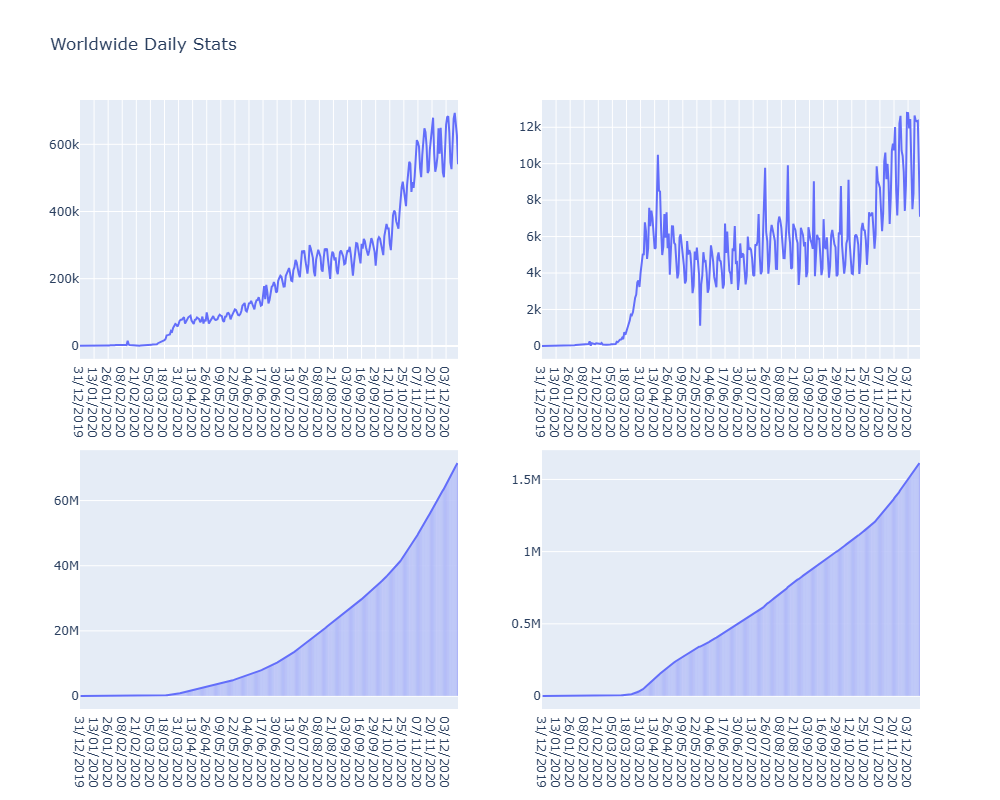
\includegraphics{./figures/mongodb/mongodb_worldwide_daily_stats.png}
\caption{MongoDB: time series and barplot+line combinesd plots showing
in the first row the daily cases and deaths worldwide, and in the second
row the cumulative cases and deaths worldwide}
\end{figure}

The time series plots above show the daily and cumulative cases and
deaths worldwide over time. We can see that there are several waves of
cases and deaths, with peaks occurring at different times, as it was at
the start of the pandamic, the trend shows an increase glovally in cases
and deaths, this is pronouced in the cumulative plost, where the
derivative (slope) of the curve is itself increasing with time.

\hypertarget{query-5-casesdeath-weekly-analysis}{%
\paragraph{3.5 Query 5: cases/death weekly
analysis}\label{query-5-casesdeath-weekly-analysis}}

\textbf{about}: tracking weekly total cases and deaths worldwide, along
with average 14-day incidence rate and correlation estimate between
cases and deaths\\
\textbf{how?}: using mongodb aggregation, will group by ISO week and
year to get weekly total cases/deaths, average incidence rate, and
correlation estimate using the formula: corr(cases, deaths) =
E{[}cases*deaths{]} / (E{[}cases{]} * E{[}deaths{]})\\
\textbf{aim}: get a weekly overview of the pandemic situation worldwide,
also, what is interesting is something called \emph{case fatality
analysis} which aims to find correlation between the number of cases and
the number of deaths, this can help in predicting the number of deaths
based on the number of cases, useful for health authorities to plan
resources accordingly

\begin{quote}
whats new: grouping by ISO week and year using \texttt{\$isoWeek} and
\texttt{\$isoWeekYear} operators, also calculating correlation estimate
using aggregation operators and some integration of complex formulae
(was a bit hard to manage!)
\end{quote}

\begin{Shaded}
\begin{Highlighting}[]
\CommentTok{// 4) cases/death correlation analysis}
\NormalTok{weekly\_stats}\OperatorTok{=}\NormalTok{db}\OperatorTok{.}\AttributeTok{worldwide\_cases}\OperatorTok{.}\FunctionTok{aggregate}\NormalTok{([}
\NormalTok{  \{}
    \DataTypeTok{$group}\OperatorTok{:}\NormalTok{ \{}
      \DataTypeTok{\_id}\OperatorTok{:}\NormalTok{ \{}
        \DataTypeTok{year}\OperatorTok{:}\NormalTok{ \{ }\DataTypeTok{$isoWeekYear}\OperatorTok{:} \StringTok{"$date"}\NormalTok{ \}}\OperatorTok{,}
        \DataTypeTok{week}\OperatorTok{:}\NormalTok{ \{ }\DataTypeTok{$isoWeek}\OperatorTok{:} \StringTok{"$date"}\NormalTok{ \}}
\NormalTok{      \}}\OperatorTok{,}
      \DataTypeTok{weeklyCases}\OperatorTok{:}\NormalTok{ \{ }\DataTypeTok{$sum}\OperatorTok{:} \StringTok{"$cases"}\NormalTok{ \}}\OperatorTok{,}
      \DataTypeTok{weeklyDeaths}\OperatorTok{:}\NormalTok{ \{ }\DataTypeTok{$sum}\OperatorTok{:} \StringTok{"$deaths"}\NormalTok{ \}}\OperatorTok{,}
      \DataTypeTok{weekly14DayIncidence}\OperatorTok{:}\NormalTok{ \{ }\DataTypeTok{$avg}\OperatorTok{:} \StringTok{"$Cumulative\_number\_for\_14\_days\_of\_COVID{-}19\_cases\_per\_100000"}\NormalTok{ \}}\OperatorTok{,}
      \DataTypeTok{corr}\OperatorTok{:}\NormalTok{ \{ }\DataTypeTok{$avg}\OperatorTok{:}\NormalTok{ \{ }\DataTypeTok{$multiply}\OperatorTok{:}\NormalTok{ [}\StringTok{"$cases"}\OperatorTok{,} \StringTok{"$deaths"}\NormalTok{] \}  \}}
\NormalTok{    \}}
\NormalTok{  \}}\OperatorTok{,}
\NormalTok{  \{}
    \DataTypeTok{$project}\OperatorTok{:}\NormalTok{ \{}
      \DataTypeTok{year}\OperatorTok{:} \StringTok{"$\_id.year"}\OperatorTok{,}
      \DataTypeTok{week}\OperatorTok{:} \StringTok{"$\_id.week"}\OperatorTok{,}
      \DataTypeTok{weeklyCases}\OperatorTok{:} \DecValTok{1}\OperatorTok{,}
      \DataTypeTok{weeklyDeaths}\OperatorTok{:} \DecValTok{1}\OperatorTok{,}
      \DataTypeTok{weekly14DayIncidence}\OperatorTok{:} \DecValTok{1}\OperatorTok{,}
      \DataTypeTok{correlationEstimate}\OperatorTok{:}\NormalTok{ \{}
        \DataTypeTok{$cond}\OperatorTok{:}\NormalTok{ [}
\NormalTok{          \{ }\DataTypeTok{$eq}\OperatorTok{:}\NormalTok{ [\{ }\DataTypeTok{$multiply}\OperatorTok{:}\NormalTok{ [}\StringTok{"$weeklyCases"}\OperatorTok{,} \StringTok{"$weeklyDeaths"}\NormalTok{] \}}\OperatorTok{,} \DecValTok{0}\NormalTok{] \}}\OperatorTok{,}
          \KeywordTok{null}\OperatorTok{,}
\NormalTok{          \{ }\DataTypeTok{$divide}\OperatorTok{:}\NormalTok{ [}\StringTok{"$corr"}\OperatorTok{,}\NormalTok{ \{ }\DataTypeTok{$multiply}\OperatorTok{:}\NormalTok{ [}\StringTok{"$weeklyCases"}\OperatorTok{,} \StringTok{"$weeklyDeaths"}\NormalTok{] \}] \}}
\NormalTok{        ]}
\NormalTok{      \}}\OperatorTok{,}
      \DataTypeTok{\_id}\OperatorTok{:} \DecValTok{0}
\NormalTok{    \}}
\NormalTok{  \}}\OperatorTok{,}
\NormalTok{  \{ }\DataTypeTok{$sort}\OperatorTok{:}\NormalTok{ \{ }\DataTypeTok{year}\OperatorTok{:} \DecValTok{1}\OperatorTok{,} \DataTypeTok{week}\OperatorTok{:} \DecValTok{1}\NormalTok{ \} \}}
\NormalTok{])}
\end{Highlighting}
\end{Shaded}

result:

\begin{itemize}
\tightlist
\item
  \texttt{year}: ISO week year
\item
  \texttt{week}: ISO week number
\item
  \texttt{weeklyCases}: total number of cases worldwide in that week
\item
  \texttt{weeklyDeaths}: total number of deaths worldwide in that week
\item
  \texttt{weekly14DayIncidence}: average 14-day incidence rate worldwide
  in that week
\item
  \texttt{correlationEstimate}: estimate of correlation between cases
  and deaths in that week
\end{itemize}

\begin{figure}
\centering
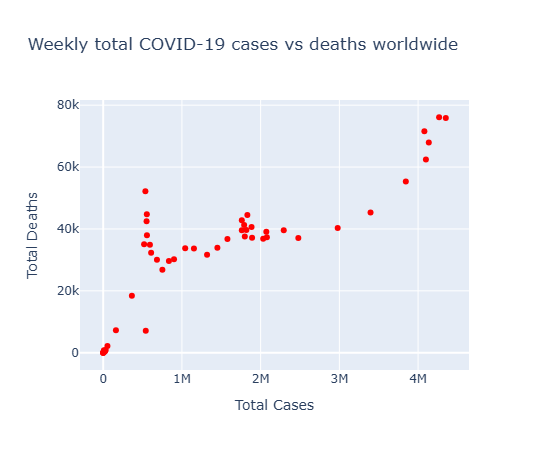
\includegraphics{./figures/mongodb/mongodb_cases_vs_deaths.png}
\caption{MongoDB: weekly scatterplot of sum of deaths vs sum of cases}
\end{figure}

This is a common analysis done in epidemiology to understand the
relationship between the number of cases and the number of deaths. A
high correlation estimate indicates that there is a strong relationship
between the two variables, meaning that as the number of cases
increases, the number of deaths also tends to increase (can be useful
for predicting the number of deaths based on the number of cases, which
can help health authorities plan resources accordingly)

\hypertarget{query-6-collect-the-14-day-incidence-rate-worldwide-per-day-for-these-2-dates-group-by-country}{%
\paragraph{3.6 Query 6: collect the 14-day incidence rate worldwide per
day for these 2 dates, group by
country}\label{query-6-collect-the-14-day-incidence-rate-worldwide-per-day-for-these-2-dates-group-by-country}}

\textbf{about}: collecting the 14-day incidence rate worldwide per day
for the earliest and latest dates in the dataset, grouped by country\\
\textbf{how?}: using mongodb queries to find the earliest and latest
dates, then colelcting the incidence rates for those dates across all
entries (one entry per country in a day actually)\\
\textbf{aim}: get a snapshot of the incidence rates at the start and end
of the dataset, useful for comparing how the situation has evolved over
time across countries. It's actually interesting if one wants to test
significance of change between 2 dates, while this might not be ideal in
this dataset (doesnt span over a long period of time), the idea od
performing statistical analysis still holds (boxplots and comparisons)

\begin{Shaded}
\begin{Highlighting}[]
\CommentTok{// 5) collect the 14{-}day incidence rate worldwide per day for these 2 dates, group by country}
\NormalTok{earliest\_date}\OperatorTok{=}\NormalTok{db}\OperatorTok{.}\AttributeTok{worldwide\_cases}\OperatorTok{.}\FunctionTok{find}\NormalTok{()}\OperatorTok{.}\FunctionTok{sort}\NormalTok{(\{ }\DataTypeTok{date}\OperatorTok{:} \DecValTok{1}\NormalTok{ \})}\OperatorTok{.}\FunctionTok{limit}\NormalTok{(}\DecValTok{1}\NormalTok{)}\OperatorTok{.}\FunctionTok{next}\NormalTok{()}
\NormalTok{latest\_date}\OperatorTok{=}\NormalTok{db}\OperatorTok{.}\AttributeTok{worldwide\_cases}\OperatorTok{.}\FunctionTok{find}\NormalTok{()}\OperatorTok{.}\FunctionTok{sort}\NormalTok{(\{ }\DataTypeTok{date}\OperatorTok{:} \OperatorTok{{-}}\DecValTok{1}\NormalTok{ \})}\OperatorTok{.}\FunctionTok{limit}\NormalTok{(}\DecValTok{1}\NormalTok{)}\OperatorTok{.}\FunctionTok{next}\NormalTok{()}

\NormalTok{start\_end\_date\_incidence\_stats}\OperatorTok{=}\NormalTok{db}\OperatorTok{.}\AttributeTok{worldwide\_cases}\OperatorTok{.}\FunctionTok{find}\NormalTok{(}
\NormalTok{  \{ }\DataTypeTok{dateRep}\OperatorTok{:}\NormalTok{ \{ }\DataTypeTok{$in}\OperatorTok{:}\NormalTok{ [ earliest\_date}\OperatorTok{.}\AttributeTok{dateRep}\OperatorTok{,}\NormalTok{ latest\_date}\OperatorTok{.}\AttributeTok{dateRep}\NormalTok{ ] \} \}}\OperatorTok{,}
\NormalTok{  \{ }\DataTypeTok{countriesAndTerritories}\OperatorTok{:} \DecValTok{1}\OperatorTok{,} \DataTypeTok{geoId}\OperatorTok{:} \DecValTok{1}\OperatorTok{,} \DataTypeTok{dateRep}\OperatorTok{:} \DecValTok{1}\OperatorTok{,}
    \StringTok{"Cumulative\_number\_for\_14\_days\_of\_COVID{-}19\_cases\_per\_100000"}\OperatorTok{:} \DecValTok{1}\OperatorTok{,}
     \DataTypeTok{\_id}\OperatorTok{:} \DecValTok{0} 
\NormalTok{  \}}
\NormalTok{)}
\end{Highlighting}
\end{Shaded}

result:

\begin{itemize}
\tightlist
\item
  \texttt{countriesAndTerritories}: country name
\item
  \texttt{geoId}: country geo id
\item
  \texttt{dateRep}: date (day)
\item
  \texttt{Cumulative\_number\_for\_14\_days\_of\_COVID-19\_cases\_per\_100000}:
  14-day incidence rate for that country on that date
\end{itemize}

\begin{figure}
\centering
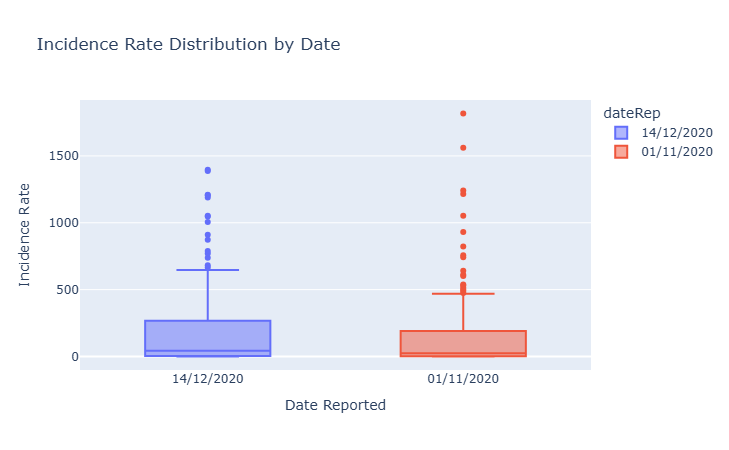
\includegraphics{./figures/mongodb/mongodb_box.png}
\caption{MongoDB: boxplot showing distribution of 14-day incidence rates
worldwide per country for the earliest and latest dates in the dataset}
\end{figure}

This can be useful to compare between 2 timepoints, boxplots will
relveal distribution, based on which would be a statistical test to
compare the 2 distributions (t-test, mann-whitney, etc.)

\hypertarget{hadoop}{%
\subsection{Hadoop}\label{hadoop}}

\hypertarget{setup-1}{%
\subsubsection{1. setup}\label{setup-1}}

Creating a hadoop container using the pulled image, then moving the
mapper and reducer scripts into the container

\begin{Shaded}
\begin{Highlighting}[]
\ExtensionTok{docker}\NormalTok{ run }\AttributeTok{{-}it} \AttributeTok{{-}{-}name}\NormalTok{ bigdata\_hadoop prasanthj/docker{-}hadoop /etc/bootstrap.sh }\AttributeTok{{-}bash}
\CommentTok{\# docker start {-}i bigdata\_hadoop}
\end{Highlighting}
\end{Shaded}

\begin{Shaded}
\begin{Highlighting}[]
\ExtensionTok{docker}\NormalTok{ cp code/scripts/reducers/ bigdata\_hadoop:/}
 \ExtensionTok{docker}\NormalTok{ cp code/scripts/mappers bigdata\_hadoop:/}
\end{Highlighting}
\end{Shaded}

\emph{now inside the container}

\begin{Shaded}
\begin{Highlighting}[]
\ExtensionTok{jps}
\BuiltInTok{export} \VariableTok{PATH}\OperatorTok{=}\VariableTok{$PATH}\NormalTok{:}\VariableTok{$HADOOP\_PREFIX}\NormalTok{/bin }\OperatorTok{\textgreater{}\textgreater{}}\NormalTok{ \textasciitilde{}/.bashrc}
\BuiltInTok{source}\NormalTok{ \textasciitilde{}/.bashrc}
\ExtensionTok{hadoop}\NormalTok{ version}
\end{Highlighting}
\end{Shaded}

\hypertarget{data-preperation-1}{%
\subsubsection{2. data preperation}\label{data-preperation-1}}

\begin{Shaded}
\begin{Highlighting}[]
\ExtensionTok{curl}\NormalTok{ https://opendata.ecdc.europa.eu/covid19/casedistribution/csv/data.csv }\AttributeTok{{-}o}\NormalTok{ data/covid.csv}
\FunctionTok{wc} \AttributeTok{{-}l}\NormalTok{ data/covid.csv }
\CommentTok{\# 61901 covid.csv}
\end{Highlighting}
\end{Shaded}

\emph{the 1 is for the extra header file: same as the json data taken in
mongodb}

\begin{quote}
we will check if the datasets are different later on after processing
\end{quote}

\begin{Shaded}
\begin{Highlighting}[]
\ExtensionTok{hdfs}\NormalTok{ dfs }\AttributeTok{{-}put}\NormalTok{ data/covid.csv covid.csv}
\FunctionTok{mkdir}\NormalTok{ output/}
\FunctionTok{mkdir}\NormalTok{ logs/ }\CommentTok{\# {-}{-} to save logs of hadoop jobs}
\end{Highlighting}
\end{Shaded}

So in here will:

\begin{itemize}
\tightlist
\item
  create output csv files resulting from mapreduce jobs
\item
  create logs directory to save logs of hadoop jobs for later analysis
  (performance comparison with mongodb)
\end{itemize}

\hypertarget{queries}{%
\subsubsection{3. Queries}\label{queries}}

\hypertarget{query-1-continent-stat}{%
\paragraph{3.1 Query 1: continent stat}\label{query-1-continent-stat}}

\begin{Shaded}
\begin{Highlighting}[]
\ExtensionTok{hadoop}\NormalTok{ jar }\VariableTok{$HADOOP\_COMMON\_HOME}\NormalTok{/share/hadoop/tools/lib/hadoop{-}streaming{-}2.7.2.jar }\DataTypeTok{\textbackslash{}}
\NormalTok{{-}D mapreduce.job.name=}\StringTok{"continent\_stats"} \DataTypeTok{\textbackslash{}}
\NormalTok{{-}files mappers/continent\_stats\_mapper.py,reducers/continent\_stats\_reducer.py }\DataTypeTok{\textbackslash{}}
\NormalTok{{-}input covid.csv }\DataTypeTok{\textbackslash{}}
\NormalTok{{-}output continent\_stats/ }\OperatorTok{\textgreater{}}\NormalTok{ logs/continent\_stats.log }\DecValTok{2}\OperatorTok{\textgreater{}\&}\DecValTok{1}
\end{Highlighting}
\end{Shaded}

\begin{Shaded}
\begin{Highlighting}[]
\ExtensionTok{hdfs}\NormalTok{ dfs }\AttributeTok{{-}cat}\NormalTok{ continent\_stats/}\PreprocessorTok{*}  \OperatorTok{\textgreater{}}\NormalTok{ output/continent\_stats.csv}
\end{Highlighting}
\end{Shaded}

\begin{figure}
\centering
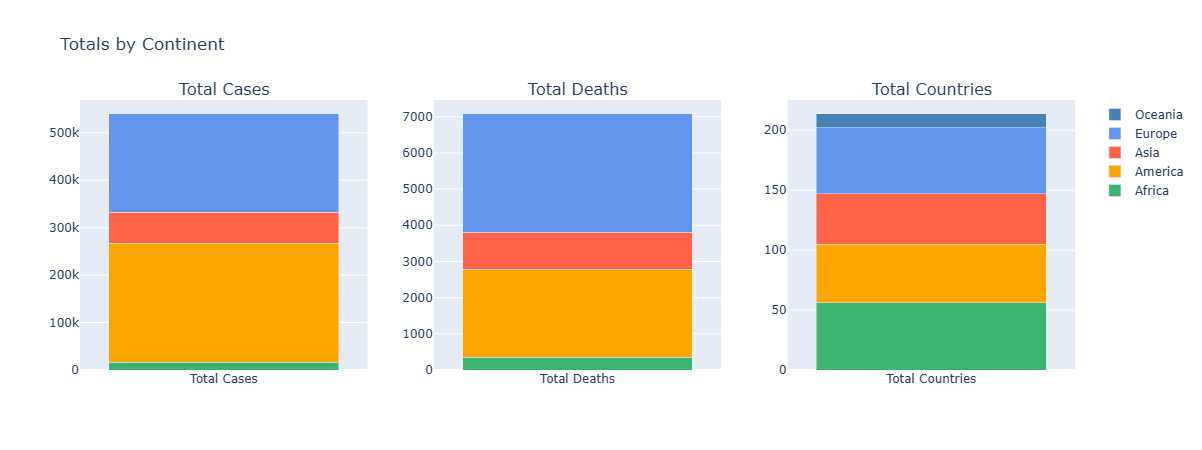
\includegraphics{./figures/hadoop/hadoop_bar_stacked_by_continent.png}
\caption{Hadoop: Stacked bar plot showing distribution accross
continents}
\end{figure}

Similar trend as before with mongodb, Europe and North America most
affected, Africa least affected, countries representation also similar

\hypertarget{query-2-country-stats}{%
\paragraph{3.2 Query 2: country stats}\label{query-2-country-stats}}

\begin{Shaded}
\begin{Highlighting}[]
\ExtensionTok{hadoop}\NormalTok{ jar }\VariableTok{$HADOOP\_COMMON\_HOME}\NormalTok{/share/hadoop/tools/lib/hadoop{-}streaming{-}2.7.2.jar }\DataTypeTok{\textbackslash{}}
\NormalTok{{-}D mapreduce.job.name=}\StringTok{"country\_stats"} \DataTypeTok{\textbackslash{}}
\NormalTok{{-}files mappers/country\_stats\_mapper.py,reducers/country\_stats\_reducer.py }\DataTypeTok{\textbackslash{}}
\NormalTok{{-}input covid.csv }\DataTypeTok{\textbackslash{}}
\NormalTok{{-}output country\_stats/ }\OperatorTok{\textgreater{}}\NormalTok{ logs/country\_stats.log }\DecValTok{2}\OperatorTok{\textgreater{}\&}\DecValTok{1}
\end{Highlighting}
\end{Shaded}

\begin{Shaded}
\begin{Highlighting}[]
\ExtensionTok{hdfs}\NormalTok{ dfs }\AttributeTok{{-}cat}\NormalTok{ country\_stats/}\PreprocessorTok{*}  \OperatorTok{\textgreater{}}\NormalTok{ output/country\_stats.csv}
\end{Highlighting}
\end{Shaded}

\begin{figure}
\centering
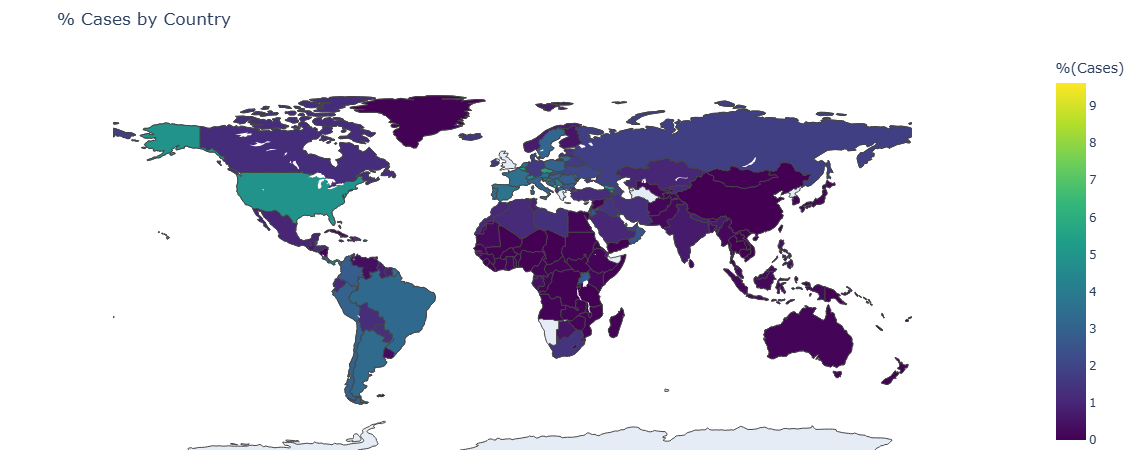
\includegraphics{./figures/hadoop/hadoop_map_cases.png}
\caption{Hadoop: map showing percentage of cases relative to population
per country}
\end{figure}

The cases map show some similarity with the one obtained with mongodb,
with some differences in color intensity for some countries but
generally we see:

\begin{itemize}
\tightlist
\item
  US and latin america highly affected
\item
  Western Europe also with lighter colors\\
\item
  Africa less overall
\end{itemize}

These discrepancies can be due to rounding errors or differences in how
the data is processed in the mapreduce jobs compared to mongodb
aggregations, as these percentages are quite small.

\begin{figure}
\centering
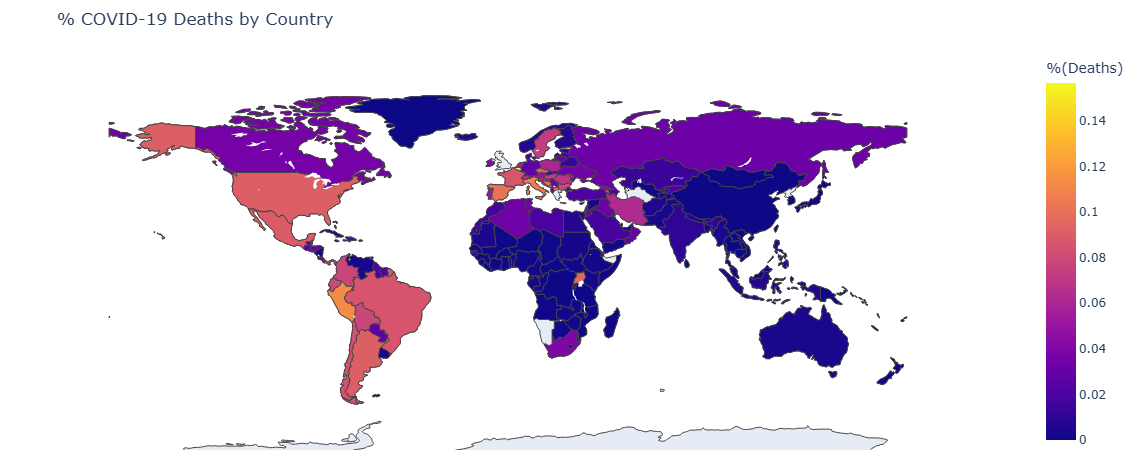
\includegraphics{./figures/hadoop/hadoop_map_deathsc.png}
\caption{Hadoop: map showing percentage of deaths relative to population
per country}
\end{figure}

Also same for deaths map, similar trends but some differences in color
intensity for some countries, overall the same observations hold.

\begin{figure}
\centering
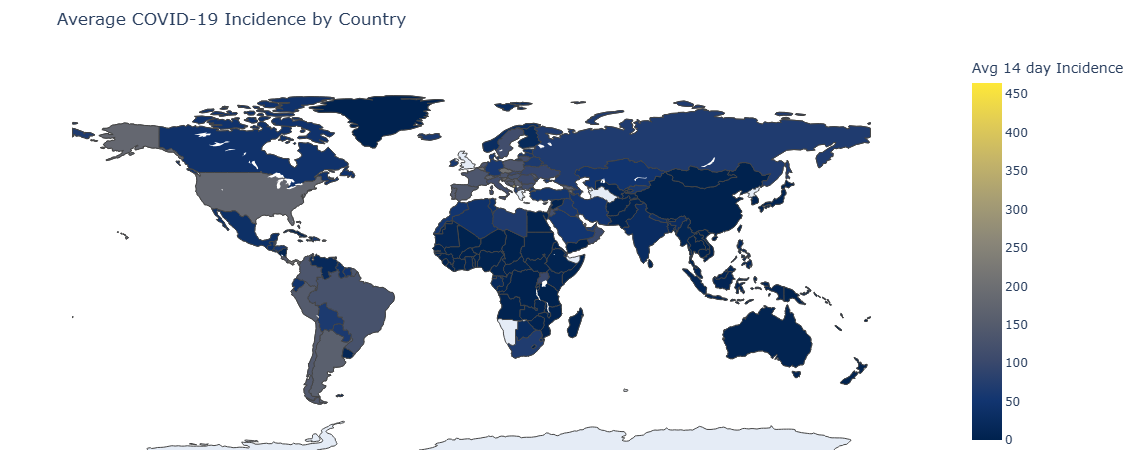
\includegraphics{./figures/hadoop/hadoop_map_incidencec.png}
\caption{Hadoop: map showing average 14-day incidence rate per country}
\end{figure}

Same for incidence rate map.

\hypertarget{query-3-usa-daily-stats-1}{%
\paragraph{3.3 Query 3: USA daily
stats}\label{query-3-usa-daily-stats-1}}

\begin{Shaded}
\begin{Highlighting}[]
\CommentTok{\# hdfs dfs {-}rm {-}r USA\_daily\_stats/}
\ExtensionTok{hadoop}\NormalTok{ jar }\VariableTok{$HADOOP\_COMMON\_HOME}\NormalTok{/share/hadoop/tools/lib/hadoop{-}streaming{-}2.7.2.jar }\DataTypeTok{\textbackslash{}}
\NormalTok{{-}D mapreduce.job.name=}\StringTok{"usa\_daily\_stats"} \DataTypeTok{\textbackslash{}}
\NormalTok{{-}files mappers/USA\_daily\_stats\_mapper.py,reducers/USA\_daily\_stats\_reducer.py  }\DataTypeTok{\textbackslash{}}
\NormalTok{{-}mapper USA\_daily\_stats\_mapper.py }\DataTypeTok{\textbackslash{}}
\NormalTok{{-}reducer USA\_daily\_stats\_reducer.py }\DataTypeTok{\textbackslash{}}
\NormalTok{{-}input covid.csv }\DataTypeTok{\textbackslash{}}
\NormalTok{{-}output USA\_daily\_stats/ }\OperatorTok{\textgreater{}}\NormalTok{ logs/USA\_daily\_stats.log }\DecValTok{2}\OperatorTok{\textgreater{}\&}\DecValTok{1}
\end{Highlighting}
\end{Shaded}

\begin{Shaded}
\begin{Highlighting}[]
\ExtensionTok{hdfs}\NormalTok{ dfs }\AttributeTok{{-}cat}\NormalTok{ USA\_daily\_stats3/}\PreprocessorTok{*} \KeywordTok{|} \FunctionTok{awk} \AttributeTok{{-}F} \StringTok{\textquotesingle{}\textbackslash{}t\textquotesingle{}} \StringTok{\textquotesingle{}\{print $2\}\textquotesingle{}} \OperatorTok{\textgreater{}}\NormalTok{ output/USA\_daily\_stats.csv}
\end{Highlighting}
\end{Shaded}

\hypertarget{query-4-worldwide-daily-stats-1}{%
\paragraph{3.4 Query 4: worldwide daily
stats}\label{query-4-worldwide-daily-stats-1}}

\begin{Shaded}
\begin{Highlighting}[]
\ExtensionTok{hadoop}\NormalTok{ jar }\VariableTok{$HADOOP\_COMMON\_HOME}\NormalTok{/share/hadoop/tools/lib/hadoop{-}streaming{-}2.7.2.jar }\DataTypeTok{\textbackslash{}}
\NormalTok{{-}D mapreduce.job.name=}\StringTok{"worldwide\_daily\_stats"} \DataTypeTok{\textbackslash{}}
\NormalTok{{-}files mappers/worldwide\_daily\_stats\_mapper.py,reducers/worldwide\_daily\_stats\_reducer.py }\DataTypeTok{\textbackslash{}}
\NormalTok{{-}mapper worldwide\_daily\_stats\_mapper.py }\DataTypeTok{\textbackslash{}}
\NormalTok{{-}reducer worldwide\_daily\_stats\_reducer.py }\DataTypeTok{\textbackslash{}}
\NormalTok{{-}input covid.csv }\DataTypeTok{\textbackslash{}}
\NormalTok{{-}output worldwide\_daily\_stats }\OperatorTok{\textgreater{}}\NormalTok{ logs/worldwide\_daily\_stats.log }\DecValTok{2}\OperatorTok{\textgreater{}\&}\DecValTok{1}
\end{Highlighting}
\end{Shaded}

\begin{Shaded}
\begin{Highlighting}[]
\ExtensionTok{hdfs}\NormalTok{ dfs }\AttributeTok{{-}cat}\NormalTok{ worldwide\_daily\_stats/}\PreprocessorTok{*}  \OperatorTok{\textgreater{}}\NormalTok{ output/worldwide\_daily\_stats.csv}
\end{Highlighting}
\end{Shaded}

\begin{figure}
\centering
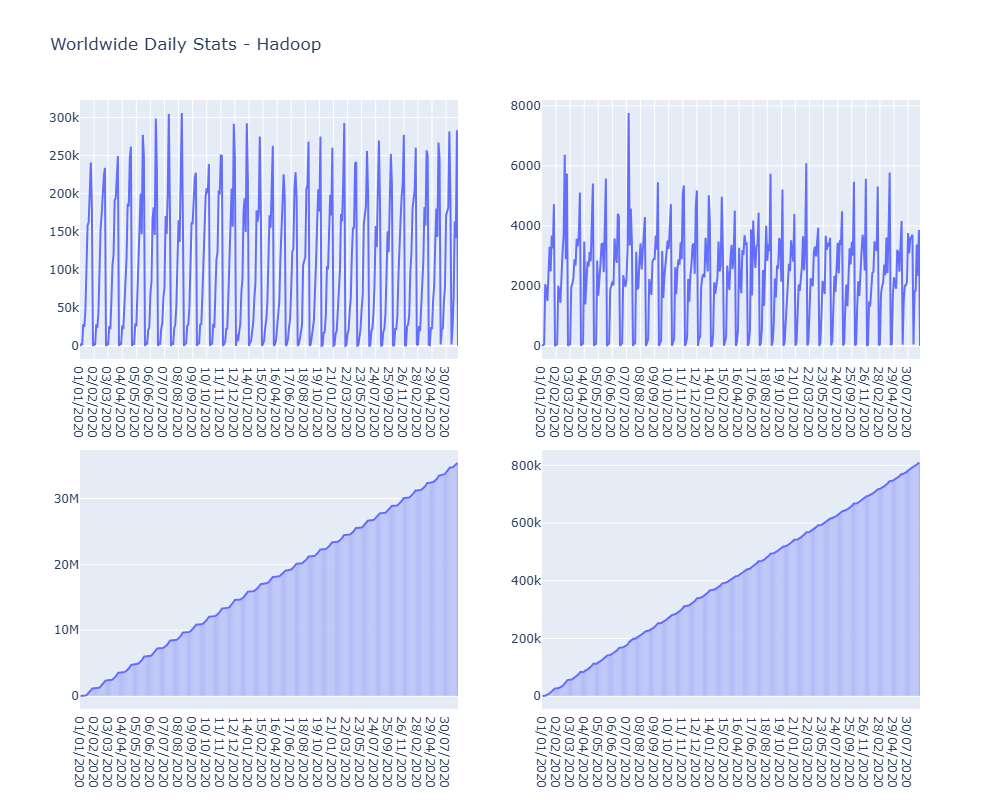
\includegraphics{./figures/hadoop/hadoop_worldwide_trendc.png}
\caption{Hadoop: time series and barplot+line combinesd plots showing in
the first row the daily cases and deaths worldwide, and in the second
row the cumulative cases and deaths worldwide}
\end{figure}

VERY IMPORTANT observation:

As we can see the worldwide trend here shows very high fluctuations
between maximal and minimal values, resembling a sinusoidal pattern -
while not particuallry epidemiologically sound, this is actually due to
reporting delays and weekly cycles in data collection and reporting.\\
It's different from results in mongodb as the datasets taken are
practically coming from different files, even if it's the same source
ansd limited to a particular number of entries (also see cumulative plot
to be \textbf{steadily} inccreasing with constant slope, which is
extremly different from the former one)

This type of plot allow to check for such anomilies in data collection
as we would be checking for daily changes in general and thus missing
entries like days or countries can be directly spotted

\hypertarget{query-5}{%
\paragraph{3.5 Query 5:}\label{query-5}}

\begin{Shaded}
\begin{Highlighting}[]
\ExtensionTok{hadoop}\NormalTok{ jar }\VariableTok{$HADOOP\_COMMON\_HOME}\NormalTok{/share/hadoop/tools/lib/hadoop{-}streaming{-}2.7.2.jar }\DataTypeTok{\textbackslash{}}
\NormalTok{{-}D mapreduce.job.name=}\StringTok{"weekly\_stats"} \DataTypeTok{\textbackslash{}}
\NormalTok{{-}files mappers/weekly\_stats\_mapper.py,reducers/weekly\_stats\_reducer.py }\DataTypeTok{\textbackslash{}}
\NormalTok{{-}mapper weekly\_stats\_mapper.py }\DataTypeTok{\textbackslash{}}
\NormalTok{{-}reducer weekly\_stats\_reducer.py }\DataTypeTok{\textbackslash{}}
\NormalTok{{-}input covid.csv }\DataTypeTok{\textbackslash{}}
\NormalTok{{-}output weekly\_stats/ }\OperatorTok{\textgreater{}}\NormalTok{ logs/weekly\_stats.log }\DecValTok{2}\OperatorTok{\textgreater{}\&}\DecValTok{1}
\end{Highlighting}
\end{Shaded}

\begin{Shaded}
\begin{Highlighting}[]
\ExtensionTok{hdfs}\NormalTok{ dfs }\AttributeTok{{-}cat}\NormalTok{ weekly\_stats/}\PreprocessorTok{*}  \OperatorTok{\textgreater{}}\NormalTok{ output/weekly\_stats.csv}
\end{Highlighting}
\end{Shaded}

\begin{figure}
\centering
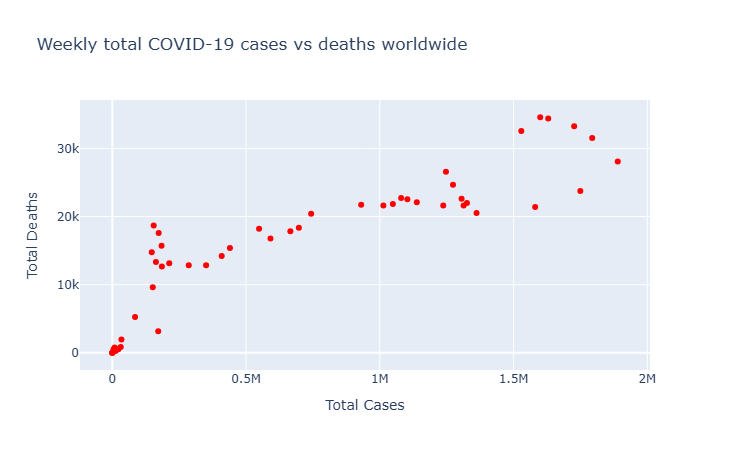
\includegraphics{./figures/hadoop/hadoopcases_vs_deathsc.png}
\caption{Hadoop: weekly scatterplot of sum of deaths vs sum of cases}
\end{figure}

The cases vs deaths plot also shows a positive correlation, similar to
mongodb, depicting important data trends.

\hypertarget{query-6}{%
\paragraph{3.6 Query 6:}\label{query-6}}

\begin{Shaded}
\begin{Highlighting}[]
\ExtensionTok{hadoop}\NormalTok{ jar }\VariableTok{$HADOOP\_COMMON\_HOME}\NormalTok{/share/hadoop/tools/lib/hadoop{-}streaming{-}2.7.2.jar }\DataTypeTok{\textbackslash{}}
\NormalTok{{-}D mapreduce.job.name=}\StringTok{"start\_end\_date\_incidence\_stats"} \DataTypeTok{\textbackslash{}}
\NormalTok{{-}files mappers/start\_end\_date\_incidence\_stats\_mapper.py,reducers/start\_end\_date\_incidence\_stats\_reducer.py }\DataTypeTok{\textbackslash{}}
\NormalTok{{-}mapper start\_end\_date\_incidence\_stats\_mapper.py }\DataTypeTok{\textbackslash{}}
\NormalTok{{-}reducer start\_end\_date\_incidence\_stats\_reducer.py }\DataTypeTok{\textbackslash{}}
\NormalTok{{-}input covid.csv }\DataTypeTok{\textbackslash{}}
\NormalTok{{-}output start\_end\_date\_incidence\_stats/ }\OperatorTok{\textgreater{}}\NormalTok{ logs/start\_end\_date\_incidence\_stats.log }\DecValTok{2}\OperatorTok{\textgreater{}\&}\DecValTok{1}
\end{Highlighting}
\end{Shaded}

\begin{Shaded}
\begin{Highlighting}[]
\ExtensionTok{hdfs}\NormalTok{ dfs }\AttributeTok{{-}cat}\NormalTok{ start\_end\_date\_incidence\_stats/}\PreprocessorTok{*}  \OperatorTok{\textgreater{}}\NormalTok{ output/start\_end\_date\_incidence\_stats.csv}
\end{Highlighting}
\end{Shaded}

\begin{figure}
\centering
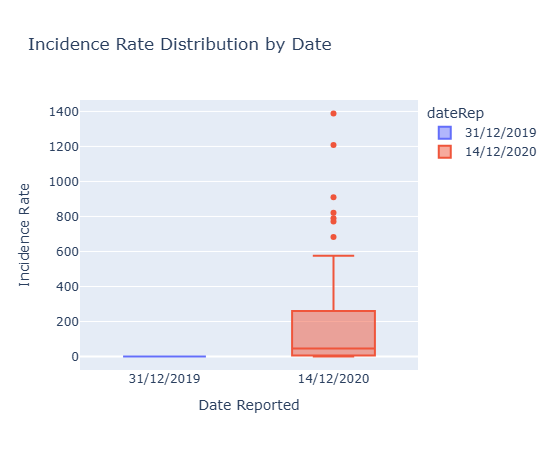
\includegraphics{./figures/hadoop/hadoop_boxplotsfi.png}
\caption{Hadoop: boxplot showing distribution of 14-day incidence rates
worldwide per country for the earliest and latest dates in the dataset}
\end{figure}

As previously seen, some days showed little to no entries in the dataset
here, leading to some discrepancies in the boxplots compared to mongodb.
In fact, one boxplot is complelty null, while not really depicting
reality, it solidifies the idea that there is missing data here, and
thus its not very plausible to perform a stat analysis using such data

\hypertarget{performance-analysis}{%
\subsection{Performance Analysis}\label{performance-analysis}}

For mongodb, we logged the performance of each query into a separate
collection called \texttt{query\_performance}, which contains the
execution time and number of documents examined for each query (you can
find it in \texttt{output/mongodb/query\_performance\_stats.json}).

For hadoop, we saved the logs of each job into the \texttt{logs/}
directory, from which we can extract the execution time and number of
input records processed for each job using this script:

\begin{Shaded}
\begin{Highlighting}[]
\ExtensionTok{python}\NormalTok{ code/scripts/process\_log.py output/hadoop/logs/ }\AttributeTok{{-}{-}output}\NormalTok{ output/hadoop/MR\_performance\_stats.csv}
\end{Highlighting}
\end{Shaded}

Will analyze the 5 main queries in terms of time, documents/records
processed and compare between the 2 tools (this analysis was performed
in \texttt{code/notebooks/performance\_analysis.ipynb})

\textbf{Time}:

\begin{figure}
\centering
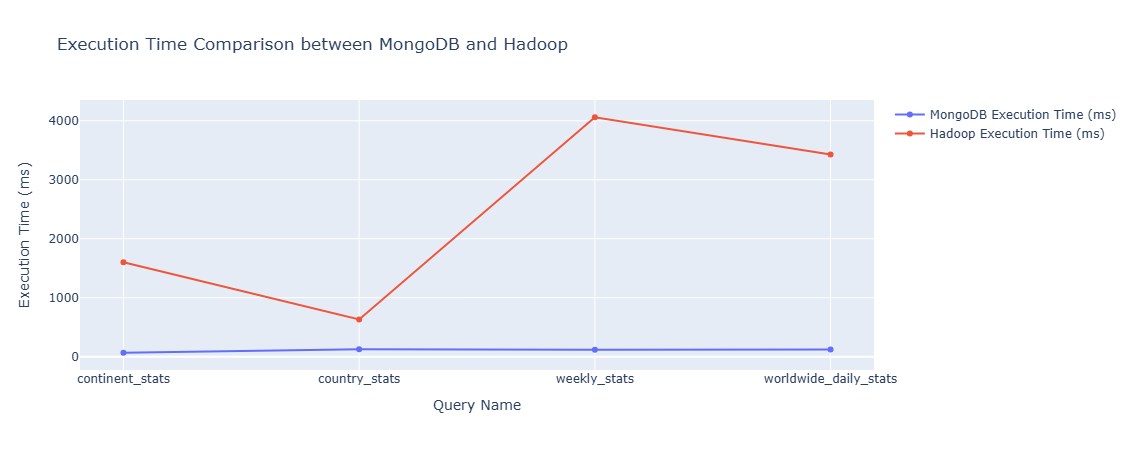
\includegraphics{./figures/time_performance.png}
\caption{line plot showing execution time comparison between mongodb and
hadoop for the main 4 queries}
\end{figure}

\emph{note, only 4 queries bcs some queries could not collected
performance stats - for example, by the way
start\_end\_date\_incidence\_stats query was implemented in mongodb, it
was a cursor not an aggregation, thus could not collect same stats as
others}

Note the big difference between the 2 tools in terms of execution time,
with mongodb being significantly faster than hadoop for all queries.
This is expected as mongodb is optimized for such aggregations and can
leverage indexes and in-memory processing, while hadoop relies on
disk-based processing and shuffling data across nodes

\textbf{Records/Documents processed}:

\begin{figure}
\centering
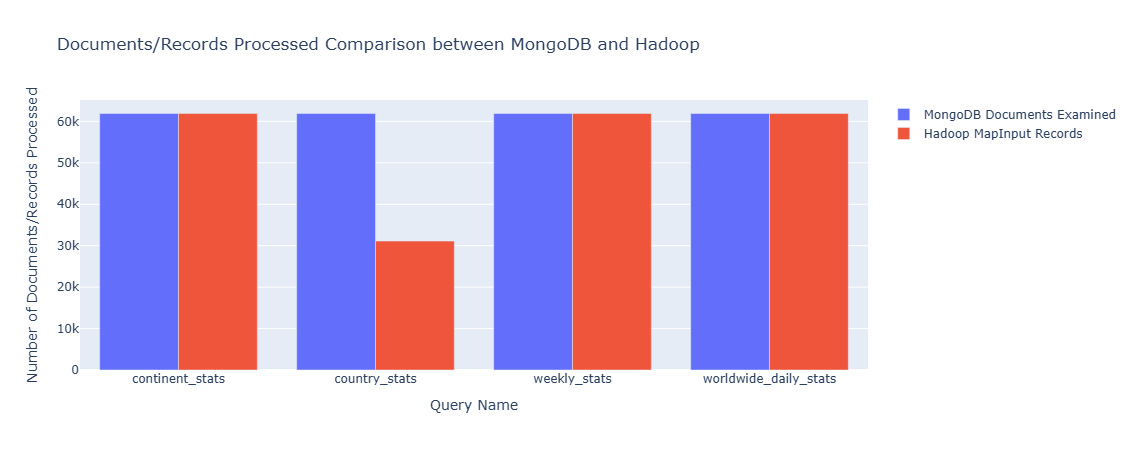
\includegraphics{./figures/processing_performance.png}
\caption{bar plot showing number of documents/records processed
comparison between mongodb and hadoop for the main 4 queries}
\end{figure}

Here, we can see that both tools processed a similar number of
records/documents for each query, with some minor differences due to the
way data is grouped and aggregated in each tool. This indicates that
both tools are capable of handling large datasets effectively, but
mongodb has an edge in terms of speed for these types of aggregations,
particularly one query was performed on significantly less in hadoop
(aggregation on query). Not the case with continents for example as it
was based on 2 aggregation stages in mongodb, thus more documents
processed.

\textbf{Some hadoop analysis}:

\begin{figure}
\centering
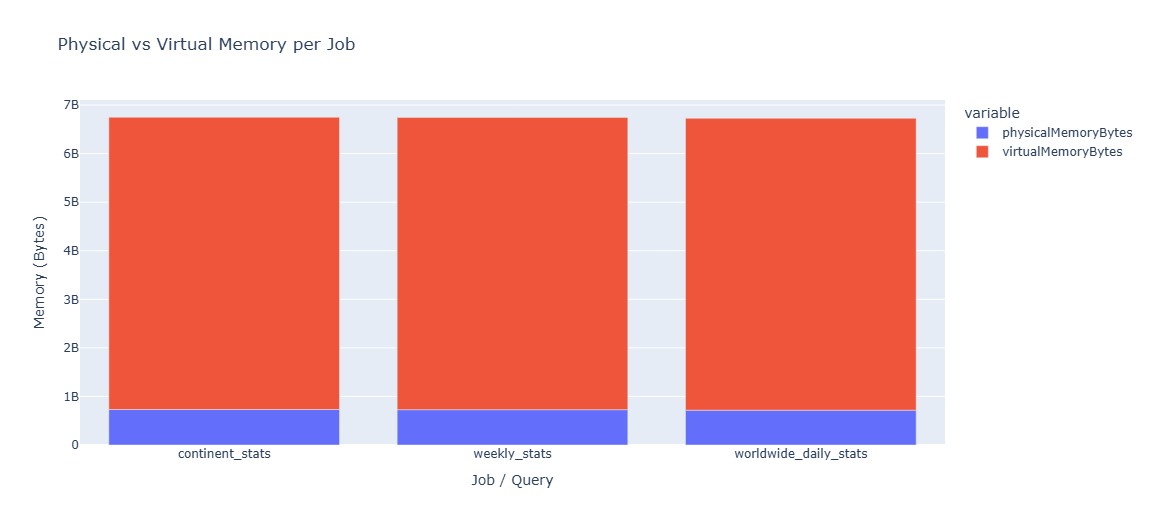
\includegraphics{./figures/phy_vs_virt.png}
\caption{Physical vs virtual memory per job}
\end{figure}

In hadoop, we can see that the physical memory used per job is
significantly lower than the virtual memory =\textgreater{} hadoop is
effectively managing memory usage and avoiding excessive swapping to
disk (important for performance, as excessive swapping can lead to
slowdowns and increased execution times)

\textbf{Closing note:} \emph{pyspark was not done by the time of
submission :'), had a couple of bugs in mapreduce that really affected
time spent on this project (the mapper file should have the word
``mapper'' in it for instance, took me more than a day to debug this
alone), working with mongodb was much more smoother and faster to
implement and test.}

Thank you for reading!

\end{document}
